% !TeX root = statnicaEKT.tex
% !TeX spellcheck = sk_SK-Slovak
\part{BPC-AE2 - Analógová elektronika 2}
%\chapter{BPC-AE2 - Analógová elektronika 2}
\begin{huge}
Otázky:
\newline
\end{huge}
\begin{enumerate}
\item Otázka - Lineární a linearizované obvody: návrh jednostupňových zesilovačů s FET; oscilátory - charakteristická rovnice, oscilační podmínka, ladění, stabilizace amplitudy; aktivní součástky - konvejory, řízené zesilovače, násobičky, transkonduktor.
\item Otázka - Spínací a tvarovací obvody: přechodné děje a přenos signálu lineární a nelineární soustavou - přenosové články, kaskáda, zpoždění, doba hrany, kompenzovaný dělič; diodové funkční měniče; tranzistorové spínače - typy, ztráty, zátěže; klopné obvody, realizace; komparátory - prahové úrovně, hystereze, realizace; generátory průběhů.
\item Otázka Operační zesilovače (vlastnosti a použití): konstrukce – diferenční pár, Millerův OZ; provoz OZ - kompenzace a korekce kmitočtové charakteristiky, nesymetrie, rychlost přeběhu, šum, napájení, ESD, ochrany.

\end{enumerate}
\newpage
\chapter{Lineárne a linearizované obvody}
\subsection{Linearizácia pri tranzistoroch}
\textit{Len pre info} - Linearizáciou sa rozumie obmedzenie alebo odstránenie nelineárnej závislosti výstupného prúdu či napätia na vstupnej veličine. Väčšinou toto robíme s použitím degradačného rezistora, ktorý berie väčšiu časť premeny napätia na prúd na seba. Pri použití degradačného rezistora však klesá maximálna dosiahnuteľná hodnota $g_m$ s rastúcim degradačným odporom, rovnako sa prejavuje šum a výrobný rozptyl súčiastiek. 
\begin{figure}[H]
\centering
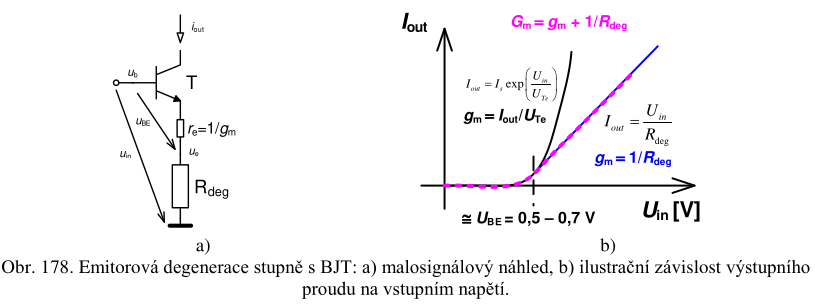
\includegraphics[width=0.7\linewidth]{Obrazky/AE2/1Otazka/linearizaciaBJT}
\caption{Závislosť výstupného prúdu na vstupnom napätí BJT}
\label{fig:linearizaciabjt}
\end{figure}
\begin{figure}[H]
\centering
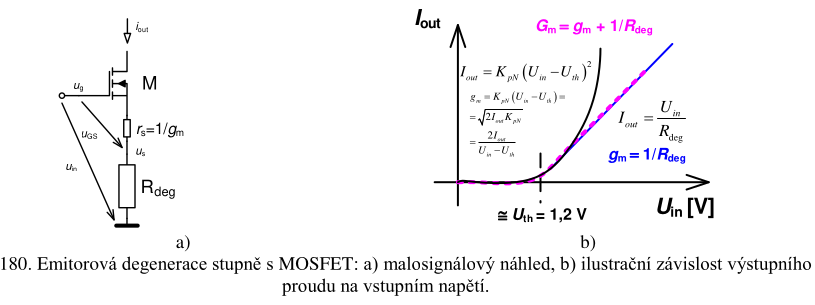
\includegraphics[width=0.7\linewidth]{Obrazky/AE2/1Otazka/linearizaciaMOSFET}
\caption{Závislosť výstupného prúdu na vstupnom napätí MOSFET}
\label{fig:linearizaciamosfet}
\end{figure}
\section{Základné parametre pre JFET a MOSFET}
\subsection{JFET}
\begin{itemize}
\item Kanál existuje aj bez $U_{GS}$ napätia
\item Pracuje v ochudzovacom režime $\rightarrow$ s $U_{GS}$ sa kanál zmenšuje $\rightarrow$ pri $U_{GS_{OFF}}$ kanál zaniká
\item maximálny prúd $I_{DSS}$ je pri nepripojenom napätí $U_{GS}$
\item \textbf{Výhody JFET}
\begin{itemize}
	\item Vysoký vstupný odpor
	\item Menší vplyv šumu
	\item Vysoký výkonový zisk
	\item Negatívny teplotný koeficient odporu $\rightarrow$ s rastúcou teplotou klesá odpor kanálu
\end{itemize}
\item \textbf{Nevýhody JFET}
\begin{itemize}
	\item Silne nelineárny
	\item Vysoké tolerancie parametrov $\rightarrow$ ťažký návrh pre niektoré aplikácie
\end{itemize}
\end{itemize}
\subsection{MOSFET}
\begin{itemize}
\item Kanál bez priloženého napätia $U_{GS}$ neexistuje
\item Pracuje v obohacovacom režime $\rightarrow$ s rastúcim $U_{GS}$ $\rightarrow$ sa kanál zväčšuje
\item Režimy v ktorých pracuje MOSFET
\begin{itemize}
	\item \textbf{Podprahový režim - slabá inverzia}
		\subitem $U_{GS} < U_{TH}$
		\subitem Správanie ako BJT tranzistor $\rightarrow$ $I_D$ závisí na $U_{GS}$ exponencionálne
		\subitem Na piču frekvenčné vlastnosti
		\subitem Maximálna hodnota $I_D$ je rovnako na piču malá
		\subitem Veľké tolerancie a teplotný rozptyl parametrov
		\subitem Závislosť $I_D$ na $U_{GS}$ je exponenciálna: \underline{\(I_D = konst. \cdot \exp\left[\frac{U_{GS}}{n \cdot U_{Te}}\right]\)}
	\item  \textbf{Lineárny režim - odpor/trióda}
		\subitem $0 < U_{DS} < (U_{GS} - U_{TH}) = U_{DS_{SAT}}; \; U_{GS} > U_{TH}$
		\subitem Saturačné napätie $U_{DS_{SAT}}$ predstavuje hranicu medzi odporovým režimom a režimom silnej inverzie
		\subitem MOSFET pracuje ako napätím riadený odpor, vníma sa v určitých medziach lineárne
	\item \textbf{Režim silnej inverzie - saturačný režim}
		\subitem \underline{Najčastejšie používaný režim}
		\subitem Správa sa ako zdroj prúdu
		\subitem $U_{DS} > U_{DS_{SAT}} = (U_{GS} - U_{TH}) ; \; U_{GS} > U_{TH}$
		\subitem Závislosť $I_D$ na $U_{GS}$ kvadratická: \underline{\(I_D = K_P \cdot\left(U_{GS} - U_{TH}\right)^2\)}
		\subitem Veľkosť $U_{DS}$ má vplyv na rovnomernosť rozloženie nosičov náboja, s rastúcim $U_{DS}$, stúpa teda aj $I_D$, \underline{nie však ideálne} $\rightarrow$ spôsobené konečným odporom kanálu $\rightarrow$ vyjadruje sa veľkosťou koeficientu modulácie dĺžky kanálu $\lambda$, ktorý spôsobuje náklon kriviek v saturačnej oblasti, samotná $\lambda$ závisí na dĺžke kanálu \emph{L}.
		\subitem $I_D$ je možné riadiť aj \emph{BULKom} - samostatnou svorkou na tranzistore $\rightarrow$ môže to spôsobiť problémy so stabilitou $\rightarrow$ pripája sa na \emph{SOURCE}.
	\item  \textbf{Režim rýchlostnej saturácie nosičov náboja}
		\subitem \(U_{DS} >> U_{DS_{SAT}}; \; U_{GS} > U_{TH}\)
		\subitem $U_{GS}$ už nemá vplyv na transkonduktanciu $g_m$ $\rightarrow$ nedá sa riadiť $\rightarrow$ veľké hodnoty $I_D$.
		\subitem Dochádza k degradácií maximálnej rýchlosti nosičov.
\end{itemize}
\end{itemize}
\begin{figure}[H]
	\centering
	\begin{subfigure}[b]{0.48\textwidth}
		\centering
		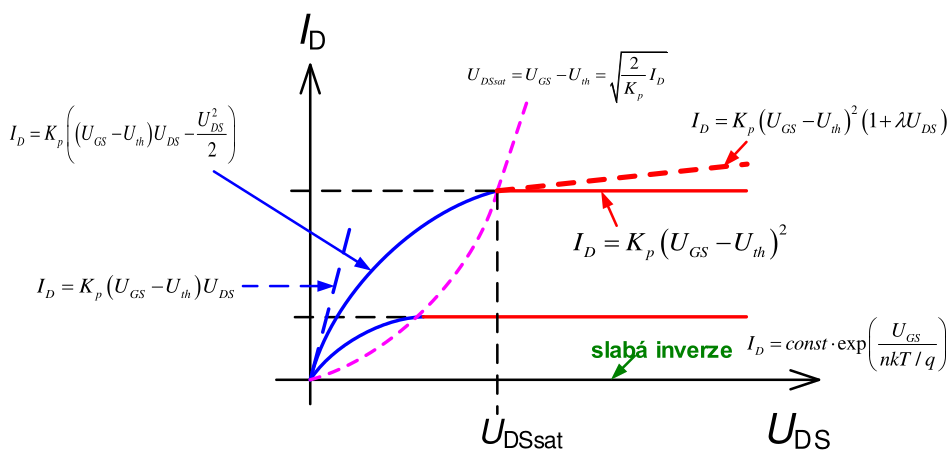
\includegraphics[width=\linewidth]{Obrazky/AE2/1Otazka/IDvsUDSMOSFET}
		\caption{Závisloť $I_D$ na $U_{DS}$}
		\label{fig:idvsudsmosfet}
	\end{subfigure}
	\begin{subfigure}[b]{0.48\textwidth}
		\centering
		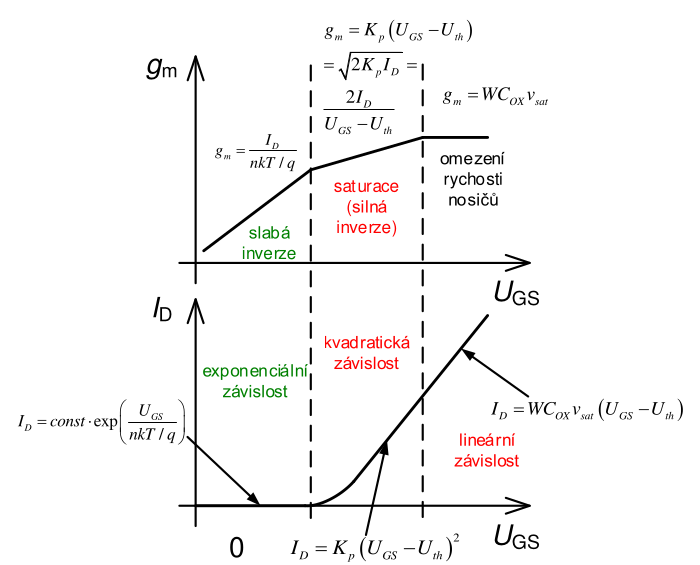
\includegraphics[width=\linewidth]{Obrazky/AE2/1Otazka/IDvsUGSMOSFET}
		\caption{Závislosť $g_m$ a $I_D$ na $U_{GS}$}
		\label{fig:idvsugsmosfet}
	\end{subfigure}
	\label{fig:prevadzkoveRezimyMosfet}
	\caption{Zhrnutie prevádzkových režimov pre MOSFET s indukovaným kanálom}
\end{figure}
\begin{figure}[H]
	\centering
	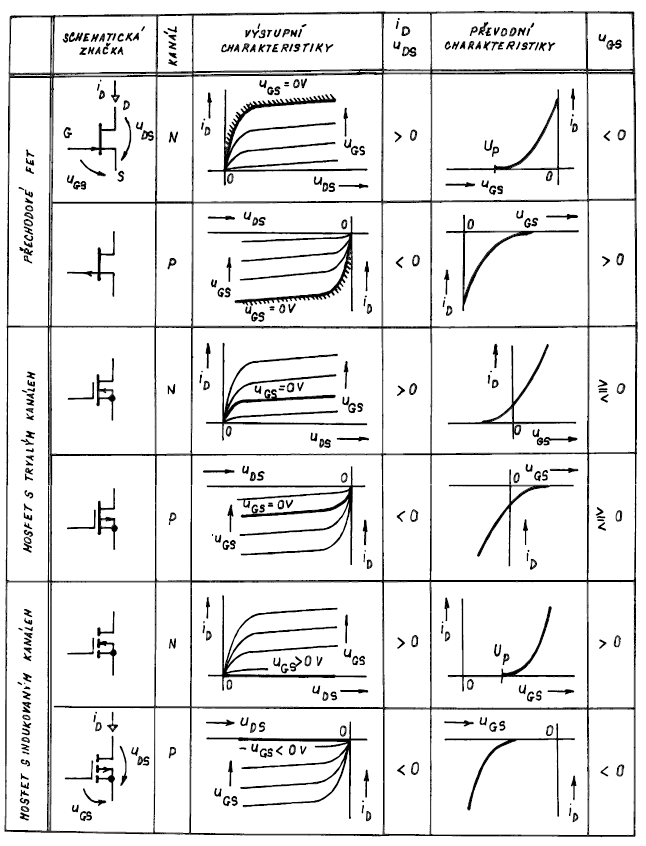
\includegraphics[width=\linewidth]{Obrazky/AE2/1Otazka/PrehladSpravaniaUnipolarov}
	\caption{Prehľad typov a správania sa rôznych unipolárnych tranzistorov}
	\label{fig:prehladspravaniaunipolarov}
\end{figure}
\newpage
\section{Návrh N-JFET zosilňovača}
\begin{figure}[H]
	
	\begin{subfigure}[b]{0.48\textwidth}
	\centering
	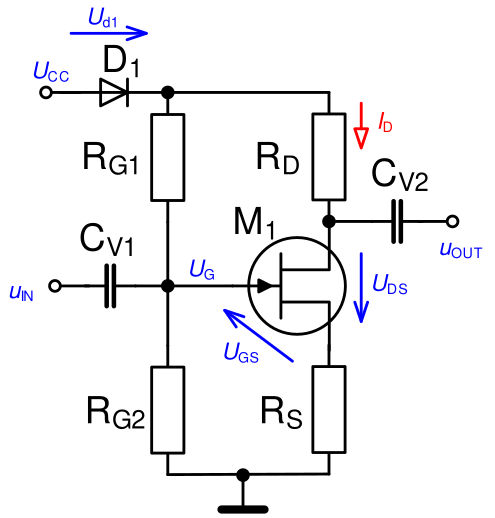
\includegraphics[width=0.7\linewidth]{Obrazky/AE2/1Otazka/NJFET-zapojenie}
	\caption{Funkčné zapojenie N-JFET zosilňovača}
	\label{fig:njfet-zapojenie}
	\end{subfigure}
	\begin{subfigure}[b]{0.48\textwidth}
	\centering
	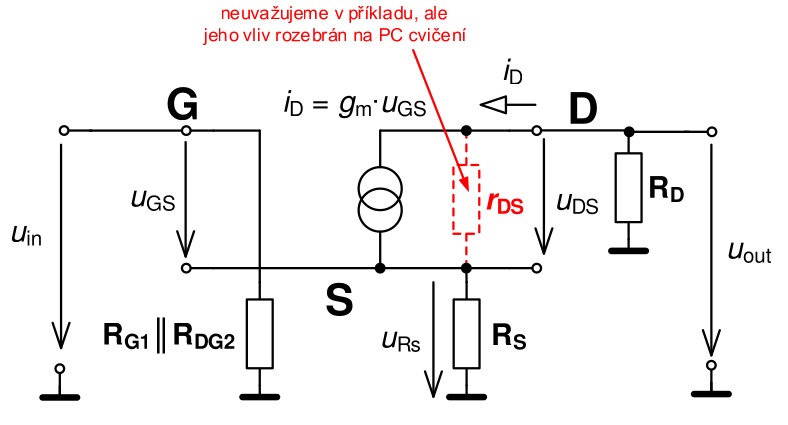
\includegraphics[width=0.7\linewidth]{Obrazky/AE2/1Otazka/NJFET-zapojenie-malosignalModel}
	\caption{Malosignálový model N-JFET zosilňovača}
	\label{fig:njfet-zapojenie-malosignalmodel}
	\end{subfigure}
\end{figure}
Približný postup návrhu:
\begin{enumerate}
	\item Potrebné zvoliť zosilnenie $K_U$ čo chceme dosiahnuť, $U_{DS}$ a $U_{GS}$ sa zvolia tak aby ležali v stredoch charakteristík pre $U_{DS}$ a $U_{GS}$.
	\item Na základe pracovného bodu sa zistia hodnoty $I_{DSS}$ a $U_{GS_{OFF}}$.
	\item Vyráta sa $I_D$, ktoré definuje kľudový pracovný bod.
	\item Zvolí sa vhodný pomer $\frac{R_D}{R_S}$.
	\item Vypočíta sa $g_m$ v pracovnom bode.
	\item Určenie hodnôt $R_S$ a $R_D$.
	\item Výpočet napätia $U_{G}$ v strede deliča.
	\item Na základe výpočtu napätia v deliči zvoliť $R_{G1}$ a dopočítať $R_{G2}$. 
	\item Výpočet väzobných kapacít $C_V$ podľa požadovanej dolnej medznej frekvencie - horná je daná JFET kapacitami - dané pomerom deliča $R_{G1}$ a $R_{G2}$ - počíta sa klasicky ako CR článok.
	\subitem Pokiaľ je známa hodnota záťaže na výstupe $R_L$, je treba ju zahrnúť a podľa nej spočítať vhodné $C_{V2}$ - uvažuje sa ako $R_D + R_L$.
	\item Pokiaľ chceme poznať výstupný rozkmit napätia musím uvažovať veľkosignálové správanie $U_{OUT}$ - ale nie je to lineárne ten výstup.
\end{enumerate}
\section{Návrh MOSFET zosilňovača}
Principiálna schéma zapojenia je rovnaká ako na \ref{fig:njfet-zapojenie}.
Narozdiel od JFET zosilňovača pri ktorom volíme pracovný bod v strede prevodových charakteristík, MOSFET musí byť v saturačnom režime na to aby fungoval ako zosilňovač.
Približný proces návrhu:
\begin{enumerate}
	\item Špecifikácia parametrov ako $I_D$, $K_U$ a podobne
	\item Určenie DC pracovného bodu do stredu oblasti saturačného režimu - sme cca v lineárnej oblasti
	\subitem Spočítať/zvoliť $I_D$
	\subitem Spočítať vstupný delič $R_{G1}$ a $R_{G2}$, $\rightarrow$ netečie tam žiaden prúd, obyčajný pomer teda
	\subitem Na základe pomeru vstupného deliča určite napätie $U_G$
	\subitem \underline{V podstate sa na základe veľko signálovej analýzy spočíta pokojový operačný bod DC}
	\item Na základe DC bodu vieme určiť transkonduktanciu skrz malosignálový model
\end{enumerate}
Keby som nevedel nič iné tak by som to zhrnul asi tak, že dôležitý je DC bod aj pri JFET a aj pri MOSFET zosilňovači.

\section{Oscilátory}
Oscilátor - Harmonický oscilátor je lienárny či linearizovaný obvod ktorý produkuje spektrálne čisté harmonické signály odvodené od funkcií sinus či cosinus. Na svoju činnosť potrebujú vždy aktívny element - tranzistor / operák / elektronku.
Podľa typu kmitajúceho okruhu delíme na:
\begin{itemize}
\item RC oscilátory - pásmo do 1MHz
\item LC oscilátory - pásmo od desiatok kHz až po stovky MHz
\begin{itemize}
	\item Dvojbodové
	\subitem Bežný Paralelný LC rezonančný obvod s paralelným záporným dynamickým odporom realizovaným tunelovou diódou - ten odtlmuje LC obvod - nahradzuje jeho straty
	\item Trojbodové 
	\subitem Colpitts
	\subitem Hartley
\end{itemize}
\item Kryštalické - jednotky až stovky MHz
\end{itemize}
RC a LC oscilátory sa dajú zjednodiť aj do skupiny \underline{Spätnoväzobných oscilátorov}.

\subsection{Popis princípu oscilátora}
Oscilátor využíva kladnú spätnú väzbu ktorá na vstup aktívneho prvku prináša výstupný signál s rovnakou fázou. Spätná väzba musí byť frekvenčne selektívna, nezáleží až tak na amplitúdovej charakteristike ale na fázovej, kmity vznikajú práve vďaka zosilneniu na aktívnom prvku. Zároveň aktívny prvok musí mať dostatočné zosilnenie na to, aby pokryl straty v pasívnej časti - spätnej väzbe. Oscilátor musí obsahovať aj obvod pre tlmenie kmitov - riadenie amplitúdy. Realizuje sa to zápornou spätnou väzbou. Riadenie amplitúdy je dôležité, aby nedošlo k saturácií výstupu. Oscilátor nepotrebuje budenie, dôsledkom zosilnenia aktívneho prvku sa vybudí sám. Pre funkciu oscilátora platia dve podmienky: Amplitúdová - hovorí o množstve energie ktorú musí dodať aktívny prvok na to aby sa pokryli straty v pasívnom obvode. Fázová - hovorí, že posuv fáze selektívnym obvodom a zosilňovačom musí byť nulový - resp násobky pi.


\begin{figure}[H]
\centering
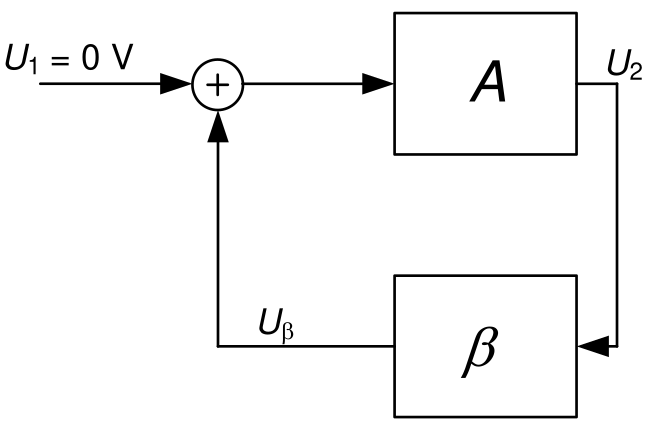
\includegraphics[width=0.35\linewidth]{Obrazky/AE2/1Otazka/principZVoscilatora}
\caption{Princíp spätnoväzobného oscilátora}
\label{fig:principzvoscilatora}
\end{figure}
\section{Oscilačné podmienky}
\begin{itemize}
\item Obvod musí byť na medzi stability
\item Korene charakteristickej rovnice musia ležať presne na Imaginárnej ose a byť komplexne združené
\item Pre prenos ZV platí Blackov vzťah: 

\begin{equation}
	K(s) = \frac{U_2}{U_1} = \frac{A}{1 \pm \beta(s)A}
\end{equation}

(Pre zápornú ZV platí, že v menovateli je +)

\item Amplitúdová podmienka: 
\begin{equation}
	\beta A = 1
\end{equation}
\item Fázová podmienka:
\begin{equation}
	\varphi_A + \varphi_\beta = 2k\pi
\end{equation}
\end{itemize}
\section{Stabilizácia amplitúdy}
Využíva sa regulačná slučka ktorá reguluje zosilnenie aktívneho prvku.
Systém Regulácie môže byť:
\begin{itemize}
\item Zotrvačný systém stabilizácie:
\begin{itemize}
	\item Zapojený zotrvačný prvok - kondenzátor C - oneskorená reakcia
	\item Funguje len na konkrétnej frekvencii
	\item Fluktuácie - časová nestabilita, fázový šum
	\item Spektrálne čistejšie - menej aktívnych prvkov
\end{itemize}
\item Nelineárny systém stabilizácie:
\begin{itemize}
	\item Vyžíva nelinearity, ktoré pre väčšie amplitúdy znížia zosilnenie (dióda)
	\item Rýchly systém
	\item Nakoľko sú tam aktívne prvky tak to má vyšší šum
\end{itemize}
\end{itemize}
\section{Charakteristická rovnica}
Získava sa pomocou riešenia obvodov cez metódy MUN, MSP. Alebo program SNAP - tam treba dať vstupný a výstupný indikátor - dáme to do miesta vysokej impedancie - v oscilátoroch tam kde je pripojený kondenzátor. V SNAPe nás zaujíma determinant admitančnej matice.

V prípade, že sme schopní identifikovať prenosy A a $\beta$ pomocou Blackovho vzťahu, potom vieme získať charakteristickú rovnicu tak, že obvod:
\begin{enumerate}
\item rozpojíme v mieste delenia $\rightarrow$ zosilňovač - spätná väzba
\item urobíme čoro-moro pri dosadzovaní do:
\begin{equation}
	1 - A\beta = 0
\end{equation}
\end{enumerate}
\section{Ladenie oscilátorov}
Oscilátor vieme ladiť zmenou hodnôt pasívnych prvkov. Ladenie je možné aj elektronicky, pri využití napríklad zosilňovača OTA, kedy zmenou transkonduktancie $g_m$ zmeníme aj frekvenciu oscilátora.
\section{Konvejory - CCII - Diamantový tranzistor}
Niekedy býva sa označuje aj ako OTA, Transkonduktor, Makrotranzistor. Jedná sa však o moderný mnohobran - principiálne prúdový Konvejor 2 generácie.


\begin{figure}[H]
\begin{subfigure}[b]{0.48\textwidth}
	\centering
	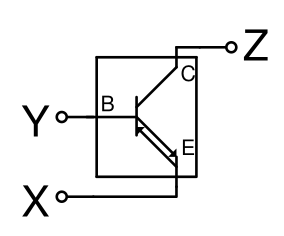
\includegraphics[width=0.5\linewidth]{Obrazky/AE2/1Otazka/diamantovyTranzistor}
	\caption{Ekvivalentné označenie brán konvejoru 2. generácie}
	\label{fig:diamantovytranzistor}
\end{subfigure}
\begin{subfigure}[b]{0.48\textwidth}
	\centering
	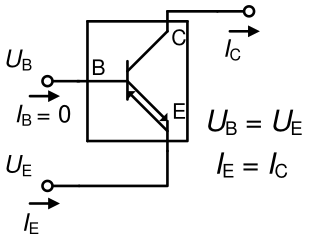
\includegraphics[width=0.5\linewidth]{Obrazky/AE2/1Otazka/PrincipKonvejora}
	\caption{Princíp Konvejora 2. generácie}
	\label{fig:principkonvejora}
\end{subfigure}
\end{figure}
\underline{Konvejorovanie: Sledovanie U a I na vstupoch, prípadne s inverziou.}

Základné vlastnosti konvejorov:
\begin{multicols}{2}
\begin{itemize}
	\item Veľká šírka pásma a rýchlosť prebehu
	\item Možnosť lineárneho nastavovania zisku prúdu medzi X a Z bránami
	\item $Z_{INP}$:
	\begin{itemize}
		\item Vstup X - vysoká impedancia
		\item Vstupy Y a Z - nízka impedancia
	\end{itemize}
	\item Horšia linearita, lepšia však ako iné OTA
	\item Nevyžadujú DC biassing
	\item Vo vnútri má zložitú štruktúru - nie je ani PNP ani NPN, z vonku je to precízny~tranzistor
	\item Nastavenie transkonduktancie pomocou degradačného rezistora v emitore $R_E$
\end{itemize}
\end{multicols}
Možné použitia:
\begin{multicols}{2}
\begin{itemize}
	\item Uzemnená báza, Vstup v emitore (svorka X), Výstup v kolektore (svorka Z) $\rightarrow$ dve zapojené takto za sebou $\rightarrow$ Sledovač prúdu
	\item Alebo v časti navrhovaného obvodu
\end{itemize}
\end{multicols}
\section{Násobičky}
\subsection{Prúdovo - napäťová násobička}
Dneska sa už nevyrába. Konkrétne napr. EL2082. Princíp tohto prvku sa však stále používa najmä vo VCA. 

Princíp činnosti: Obvod riadi prúdové zosilnenie, parameter $B_G$, pomocou riadiaceho napätia $U_G$. Dochádza k násobeniu prúdu na vstupe $X$ napätím parametrom $B_G$. Násobenie prebieha v dvoch kvadrantoch prevodovej charakteristiky. Výsledná charakteristika je lineárna a prvok je stabilný.
\begin{figure}[H]
\centering
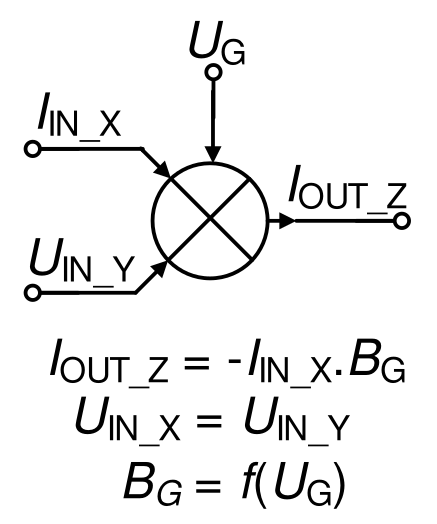
\includegraphics[width=0.15\linewidth]{Obrazky/AE2/1Otazka/principNasobickyPrudNapatie}
\caption{Princíp prúdovo - napäťovej násobičky.}
\label{fig:principnasobickyprudnapatie}
\end{figure}
\subsection{Prúdová násobička}
Podobný princíp ako Prúdovo - Napäťová násobička. Násobí výhradne vstupné prúdy. Násobenie sa deje v štyroch kvadrantoch. Napríklad prvok EL4083. Prúdový vstup $I_Z$ slúži na Biasing.
\begin{figure}[H]
\centering
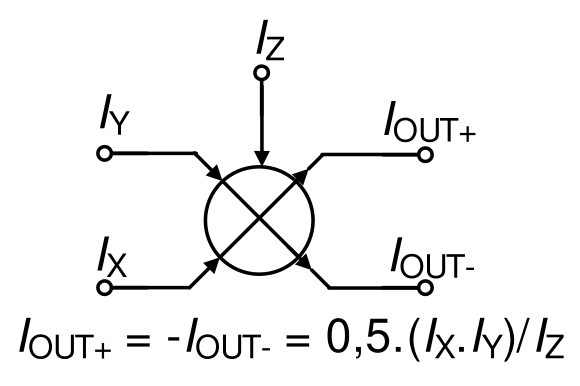
\includegraphics[width=0.35\linewidth]{Obrazky/AE2/1Otazka/prudovaNasobicka}
\caption{Symbol a princíp prúdovej násobičky}
\label{fig:prudovanasobicka}
\end{figure}
\subsection{Napäťové násobičky}
Pracuje s vstupným aj výstupným napätím (asi po zavedení spätnej väzby), násobenie prebieha v štyroch kvadrantoch. V praktických realizáciách sú vstupy plne diferenciálne, pričom je možné pripočítať vstupné napätie k výsledku násobenia. Poskytujú veľké šírky pásma. Používajú sa pre VCA, pre riadené lineárne aj nelineárne štruktúry - amplitúdové modulátory, demodulátory, obvody AGC. Prvok AD835.
\begin{figure}[H]
\centering
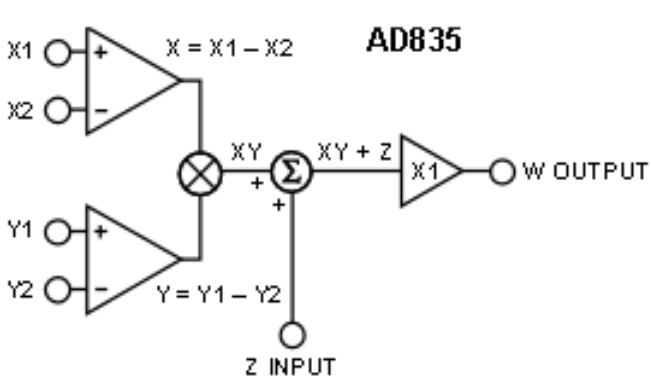
\includegraphics[width=0.35\linewidth]{Obrazky/AE2/1Otazka/napatovaNasobicka}
\caption{Napäťová násobička AD835}
\label{fig:napatovanasobicka}
\end{figure}
\section{Riadené zosilňovače}
VCA - Voltage Controlled Amplifier - možnosť riadenia zisku zosilňovača. Existuje možnosť exponenciálneho (VCA810) a aj lineárneho (VCA822) riadenia zisku.
\section{Transkonduktory - OTA}
Jedná sa o VCCS prvok. Ktorý prevádza vstupné diferenciálne napätie na výstupný prúd. Obsahuje vstupný diferenciálny zosilňovač. Rovnako ako pri iných prvkoch, aj tento je vytlačovaný a ťažko dostupný. Existujú LM13700 a LT1228. Pri ich použití je veľkým problémom veľkosť diferenciálneho vstupného napätia - dochádza k skresleniu výstupného signálu vplyvom vysokej nelinearity parametra $g_m$. Z tohoto dôvodu sa uplatňujú vstupné deliče s vysokým pomerom, bohužiaľ tieto zhoršujú šumové parametre. Nastavenie parametra $g_m$ sa robí riadiacim prúdom - to nie je práve vhodné. Problémom sú aj vstupné odpory, ktoré bývajú závislé od $g_m$ a sú celkom nízke. V púzdrach sa pridávajú aj výstupné buffre.

Parameter $g_m$ sa vytvára s pomocou biasového prúdového zrkadla.
\begin{figure}[H]
\centering
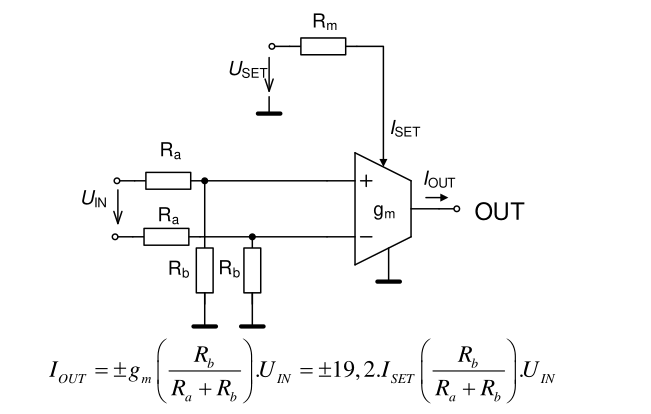
\includegraphics[width=0.5\linewidth]{Obrazky/AE2/1Otazka/zapojenieSLM13700}
\caption{Zapojenie s LM13700.}
\label{fig:zapojenieslm13700}
\end{figure}

\newpage
\chapter{Spínacie a tvarovacie obvody}
\section{Prechodové deje}
Najhoršie možné je obdĺžnikový signál / impulz - nekonečný počet harmonických zložiek $\rightarrow$ tieto signály obsahujú ostré hrany, schody a podobne $\rightarrow$ teda majú veľmi bohaté spektrum.

\textbf{Impulz:} Krátkodobá výchylka veličiny od základnej hodnoty, do ktorej sa následne vráti, jednorázová záležitosť.

\textbf{Pulz:} Opakovanie impulzov.

Pre chápanie pulzov a impulzov definujeme \textbf{typy výchyliek:} 
\begin{multicols}{2}
\begin{itemize}
	\item Jednotkový skok $\sigma$.
	\item Hodnoty:
	\begin{itemize}
		\item $\sigma = 0$ v čase $t < 0$
		\item $\sigma = 1$ v čase $t >=1$
	\end{itemize}
	\item Diracov impulz:
	\begin{itemize}
		\item Dosahuje určitej mohutnosti, je definovaný ako $\infty$ v čase $t = 0$.
		\item jedná sa o nekonečne veľký, a nekonečne úzky impulz.
		\item V praxi sa vzťahuje k jednotke.
	\end{itemize}
\end{itemize}
\end{multicols}

Reálny impulz má v prenosovej sústave exponenciálny charakter. Jednoduchá varianta je exponencionálne klesajúca tá začína jednotkovým skokom, častejšia varianta je dvojexponencionálna.

\begin{figure}[H]
\centering
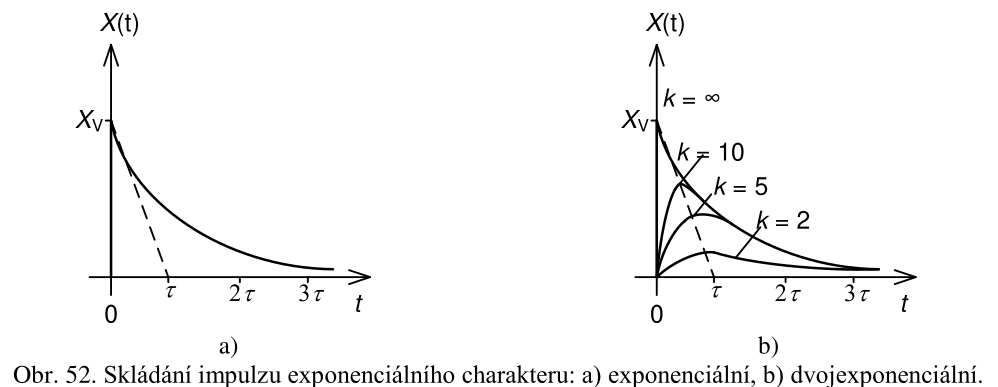
\includegraphics[width=0.6\linewidth]{Obrazky/AE2/2otazka/impulzy}
\caption{Zobrazenie impulzov.}
\label{fig:impulzy}
\end{figure}
\begin{equation}
\underset{\text{Exponenciálny impulz}}{x(t) = \sigma(t) \cdot X_V \cdot \exp\left(\frac{-t}{\tau}\right)} 
\qquad \text{a} \qquad 
\underset{\text{Dvoj-exponenciálny impulz}}{x(t) = \sigma(t) \cdot X_V \cdot \left[\exp\left(\frac{-t}{\tau}\right) - \exp\left(\frac{-k\cdot t}{\tau}\right)\right]}
\end{equation}
Kde $\tau$ predstavuje časovú konštantu - vyjadrujúcu čas potrebný pre zmenu hodnoty o \qty{63}{\%}. Či už pre pokles alebo nárast z pôvodnej hodnoty.

Prechodové deje sú popísané exponenciálnymi rovnicami. Tento popis súvisí s možnosťou transformácie správania medzi frekvenčnou a časovou oblasťou. Transformácia sa robí cez transformátorový slovník.
\begin{figure}[H]
\centering
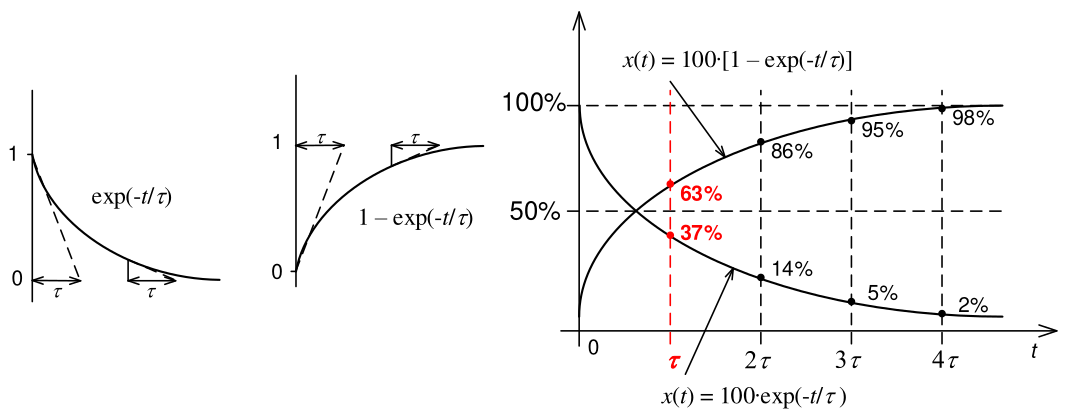
\includegraphics[width=0.7\linewidth]{Obrazky/AE2/2otazka/NormovanyPriebehExpFunkcii}
\caption{Normovaný priebeh exponenciálnych funkcií}
\label{fig:normovanypriebehexpfunkcii}
\end{figure}
Vzťah pre čas medzi dvoma úrovňami vieme definovať ako:
\begin{equation}
\Delta t = \tau \cdot \ln\left(\frac{x(\infty) - x(t_1)}{x(\infty) - x(t_2)}\right)
\end{equation}
Reálny obdĺžnikový impulz v prenosovom systéme vyzerá:
\begin{figure}[H]
\centering
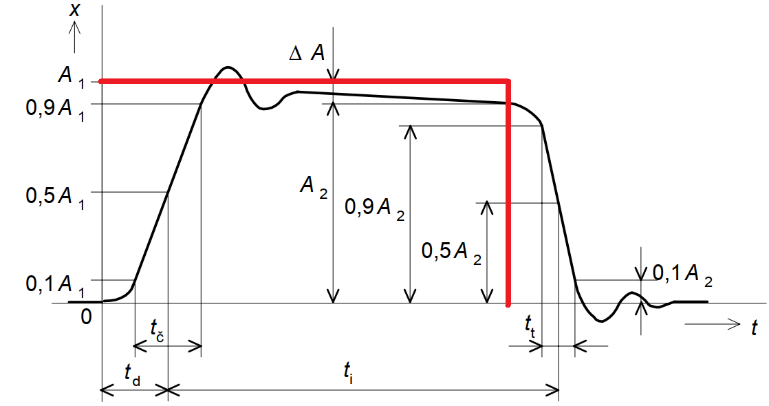
\includegraphics[width=0.7\linewidth]{Obrazky/AE2/2otazka/pravouhlyImpulz}
\caption{Porovnanie reálneho a pravoúhleho impulzu}
\label{fig:pravouhlyimpulz}
\end{figure}
Definuje sa:
\begin{itemize}
\item Doba hrany - $t_e$ resp. $t_r$ - Doba od \qty{10}{\%} po \qty{90}{\%} signálu.
\subitem \begin{equation}
	t_e = t_{0.9x} - t_{0.1x} = \tau \ln\left(\frac{x - 0,1x}{x - 0,9x}\right) = \tau \ln\left(\frac{0.1}{0.9}\right) = \tau\ln\left(9\right) \approx 2,2\tau´
\end{equation}
\item Strieda pulzu - pomer medzi aktívnou a pasívnou dobou.	
\end{itemize}
\section{Prenos lineárnou sústavou}
Lineárne články prenášajú široké spektrum frekvencií impulzov, toto spektrum je samozrejme obmedzené. Obmedzenie šírky prenášaného pásma spôsobuje lineárne skreslenie. Toto skreslenie je frekvenčne závislé, pričom nemôžu vznikať nové, pôvodne neprítomné frekvencie. V lineárnom systéme platí princíp superpozície. Signál sa oneskoruje o:
\begin{itemize}
\item Doba oneskorenia $t_d$, súvisí s lineárnym skreslením - Doba od \qty{0}{\%} po \qty{50}{\%} signálu. \textbf{Presný vzťah Platí len ak nemáme kaskádu, inak je približný.}
\subitem \begin{equation}
	t_e = t_{0.5x} - t_{0x} = \tau \ln\left(\frac{x - 0x}{x - 0,5x}\right) = \tau \ln\left(\frac{1}{0.5}\right) = \tau\ln\left(2\right) \approx 0,69\tau
	\label{eqv:38}
\end{equation}
\item Doba trvania impulzu $t_i$ - definovaná medzi \qty{50}{\%} úrovne impulzu.
\end{itemize}

Jednoduchý lineárny článok sa dá modelovať RC článkom. Definuje sa tu medzná frekvencia.
\begin{equation}
\underset{\text{Vzťah medzi dobou hrany a medznou frekvenciou.}}{t_e \approx \frac{0,35}{f_m}}
\label{eqv:teFm}
\end{equation}
Pričom doba hrany je daná vzťahom \ref{eqv:38}. Vzťah \ref{eqv:teFm} platí presne pre dolnú priepusť, približne aj pre zložitejšie obvody. Celková doba hrany bude geometrickým súčtom doby hrany článku a pôvodnej doby hrany.
\begin{equation}
t_{eo} \approx \sqrt{t_{ei}^2 + t_{e}^2} = \sqrt{t_{ei}^2 + \left(\frac{0,35}{fm}\right)^2}
\end{equation}
\subsection{Kaskáda lineárnych článkov}
Pokiaľ máme kaskádu článkov, ktoré sú od seba impedančne oddelené (Buffers), tak je to stále geometrický súčet.
\begin{figure}[H]
\centering
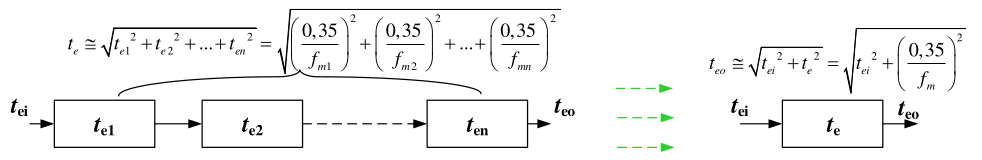
\includegraphics[width=0.9\linewidth]{Obrazky/AE2/2otazka/kaskadaClankov}
\caption{Samostatný lineárny prenosový článok a kaskáda prenosových článkov.}
\label{fig:kaskadaclankov}
\end{figure}
\begin{figure}[H]
\centering
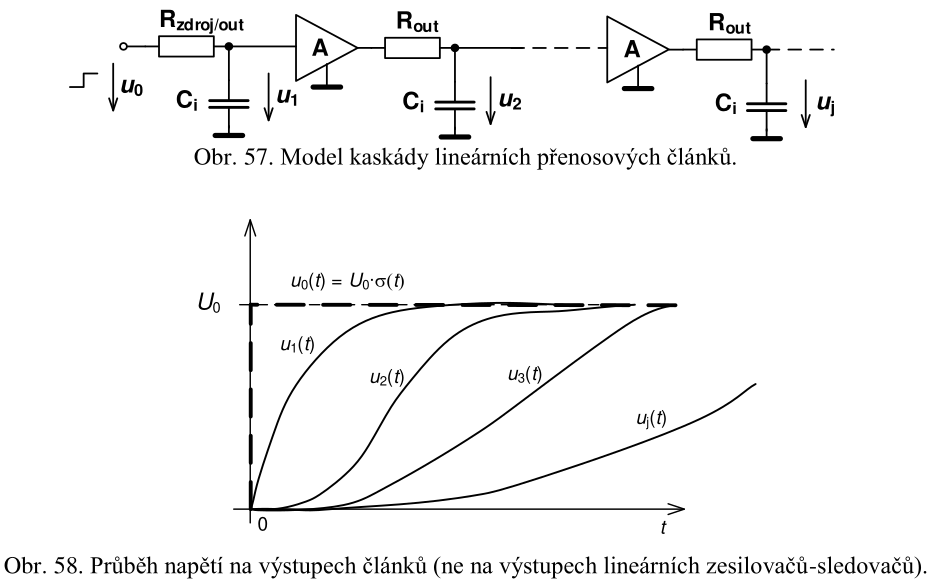
\includegraphics[width=0.7\linewidth]{Obrazky/AE2/2otazka/kaskadaClankovModel}
\caption{Model a časové priebehy článkov}
\label{fig:kaskadaclankovmodel}
\end{figure}
\textit{Poznámka: Ak jednotlivé články majú prenos iný ako 1 tak to ovplyvní aj ustálenie výstupnej úrovne kaskády.}

\section{Prenos nelineárnou sústavou}
Dochádza tu k nelineárnemu skresleniu, môžu sa objavovať nové spektrálne zložky, neplatí tu princíp superpozície. Vplývajú tu parazitné kapacity. Vlastnosti nelineárneho skreslenia:
\begin{itemize}
\item Výstupný signál obsahuje nové spektrálne zložku
\item Neplatí princíp superpozície
\item Dochádza k spojitému/nespojitému obmedzeniu signálu - prejavuje sa v nelinearite prevodnej charakteristiky
\item Dôležitý vplyv parazitných kapacít
\item Hysteréza
\end{itemize}
Vplyvom parazitných kapacít sa bude predlžovať doba hrany pôvodného signálu. Každý článok predĺži hranu. 
\underline{Maximálna dĺžka hrany je obmedzená kvôli zosilneniu!} Naopak, pokiaľ je hrana pôvodného signálu dlhá, tak po prechode kaskádou bude vplyvom zosilnenia kratkšia! Doba hrany sa po prechode niekoľkých blokov v kaskáde ustáli. $\rightarrow$ \textbf{Vlastná doba hrany}
\begin{itemize}
	\item Doba za ktorú sa ustáli doba hrany na základe relácií medzi zosilnením a zotrvačnými prvkami.
\end{itemize}

Predstava o vlastnej dobe platí len kým nedojde k rozkmitaniu zosilňovača $\rightarrow$ k tomuto dochádza pokiaľ je dĺžka pôvodnej hrany príliš veľká. Pri lineárnych prenosových článok s OZ musíme kompenzovať frekvenčnú charakteristiku zosilňovačov. Pri digitálnych sústavách stačí zaistiť dostatočne krátku hranu signálu, pri ktorých sa nemá hradlo čas rozkmitať.

\section{Integračný dvojbran - RC - dolná priepusť}
\begin{itemize}
	\item RC článok
	\item Časová konštanta: $\tau = RC$
	\item Neprenáša skokové zmeny
	\item Pri vstupnom harmonickom signále $\rightarrow$ signál fázovo posunutý o \qty{-90}{\degree} (Ak sedí frekvencia pre -3dB)
	\item Pri vstupnom obdĺžniku s kratšou periódou ako $\tau$ $\rightarrow$ výstup je trojuholník
	\item Potrebné uvažovať pripojené zariadenia - ak má zdroj signálu výstupný odpor, či záťaž článku kapacitný charakter $\rightarrow$ ovplyvňuje to $\tau$!
	\item Pokiaľ je článok zaťažený porovnateľným odporom $\rightarrow$ vytvorí sa paralelná kombinácia odporov $\rightarrow$ ovplyvní to výslednú úroveň napätia (Odporový delič) $\rightarrow$ a aj $\tau$!
\end{itemize}
\begin{figure}[H]
	\centering
	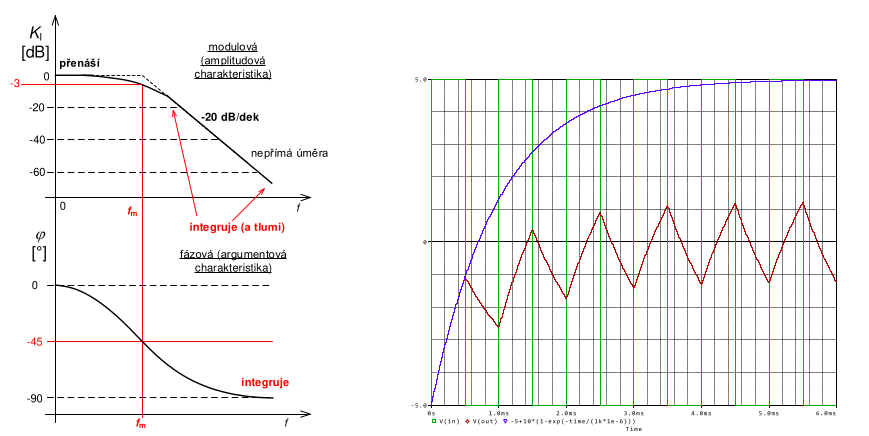
\includegraphics[width=0.7\linewidth]{Obrazky/AE2/2otazka/integracnyClanok}
	\caption{Príklad integračného procesu pre periódu vstupného signálu nižšiu ako $\tau$.}
	\label{fig:integracnyclanok}
\end{figure}
Integračný článok sa vyskytuje bežne ako forma parazity. Vytvorí sa jednoducho z výstupného odporu zdrojov a vstupných kapacít pripojených zariadení. Vytvára sa teda lineárne skreslenie signálu.

\textit{Poznámka: V prípade, že vstupný signál je hlboko v útlme \qty{-20}{dB/dec}, dochádza k stratovej integrácií $\rightarrow$ ak chceme bezstratový integrátor, musíme doplniť obvod aktívnym prvkom}
\begin{figure}[H]
	\centering
	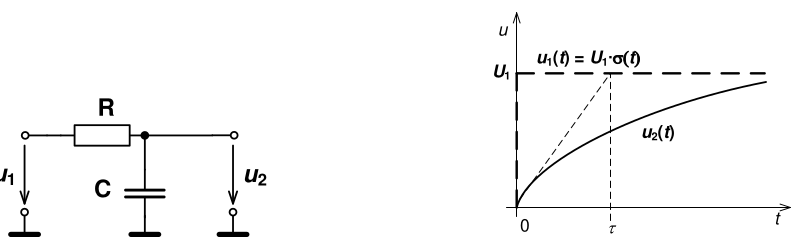
\includegraphics[width=0.7\linewidth]{Obrazky/AE2/2otazka/integracnyClanokzapojenie}
	\caption{Zapojenie integračného článku}
	\label{fig:integracnyclanokzapojenie}
\end{figure}

\section{Derivačný dvojbran - CR - horná priepusť}
\begin{itemize}
	\item CR článok
	\item Neprenáša jednosmernú zložku
	\item Časová konštanta: $\tau = CR$
	\item Pre nízke lineárne skreslenie musí byť $\tau >>$ ako šírka impulzu, čím väčší je tento rozdiel, tým kvalitnejšia derivácia.
	\item Pri vstupnom harmonickom signále $\rightarrow$ signál fázovo posunutý o \qty{90}{\degree} (Ak sedí frekvencia pre -3dB)
	\item Pri vstupnom obdĺžniku $\rightarrow$ výstup je 0 (DC zložku ee)
	\item Pri vstupnom trojuholníku $\rightarrow$ výstup je obdĺžnik
	\item \underline{Pokiaľ je zaťažený zotrvačnou záťažou, dochádza k zmene rádu článku!} (Kapacitná záťaž $\rightarrow$ Wienov článok $\rightarrow$ 2. rád)
\item Pokiaľ je pripojený na zdroj s nenulovým výstupným odporom a je k nemu pripojená rezistívna záťaž, jeho výstupné napätie je dané vytvoreným odporovým deličom.
\item Vyskutuje sa v podobe parazít medzi cestami DPS, rovnako sa s ním stretávame ako s oddeľovačom jednosmernej zložky.
\item Časová konštanta $\tau$, ovplyvňuje prenos rušivého signálu $\rightarrow$ nižžsie $\tau$, nižšie rušenie.
\end{itemize}
\textit{Poznámka: Pokiaľ sa pohybujeme v útlme, jedná sa o stratový derivačný článok}
\begin{figure}[H]
	\centering
	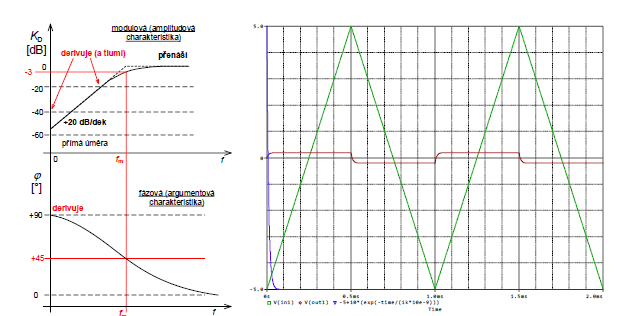
\includegraphics[width=0.7\linewidth]{Obrazky/AE2/2otazka/derivacnyClanok}
	\caption{Príklad derivačného procesu stratového derivátora}
	\label{fig:derivacnyclanok}
\end{figure}
\begin{figure}[H]
	\centering
	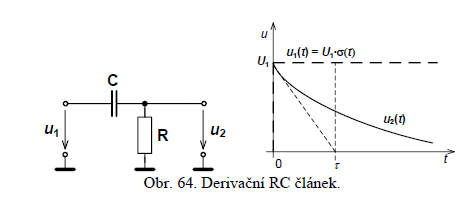
\includegraphics[width=0.7\linewidth]{Obrazky/AE2/2otazka/derivacnyClanokzapojenie}
	\caption{Zapojenie derivačného článku}
	\label{fig:derivacnyclanokzapojenie}
\end{figure}
\section{Frekvenčne závislý delič napätia}
Bavíme sa o pasívnych osciloskopických sondách.

Ideálny delič nie je frekvenčne závislý, len zníži úroveň napätia $\rightarrow$ teda nemení tvar pôvodného signálu. V realite sa však prejavuje kapacita záťaže, vznikajúca parazitnou kapacitou spojov, či vstupnou kapacitou naväzujúceho obvodu $\rightarrow$ vzniká integračný článok $\rightarrow$ delič tlmí VF zložky signálu.

Pokiaľ nechceme dopustiť toto tlmenie, musí sa delič kompenzovať. Kompenzácia sa robí paralelným kondenzátorom. Napriek tomu, to nie je obvod druhého rádu, nakoľko z pohľadu zdroja sú paralelne. Pre správne kompenzovaný delič platí, že prenos ustálenej zložky a zmeny je rovnaký \(d_R = d_C\): 
\begin{equation}
	\tau_1 = \tau_2 \implies R_1 C_1 = R_2 C_2
\end{equation}
\begin{figure}[H]
\centering
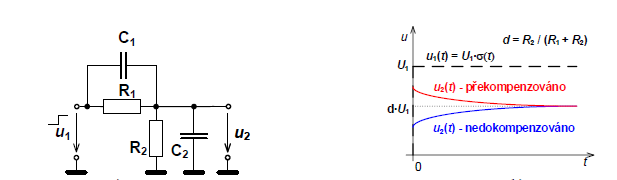
\includegraphics[width=0.7\linewidth]{Obrazky/AE2/2otazka/frekZavisDelic}
\caption{Kompenzácia deliča}
\label{fig:frekzavisdelic}
\end{figure}
V ideálnom svete, by vstupný impulz znamenal teoreticky nekonečný prúd (kondenzátory by sa museli nabiť okamžite). To však nie je možné, je to limitované výstupným odporom zdroja signálu. Vtedy sa už jedná o obvod 2. rádu.
\begin{figure}[H]
	\centering
	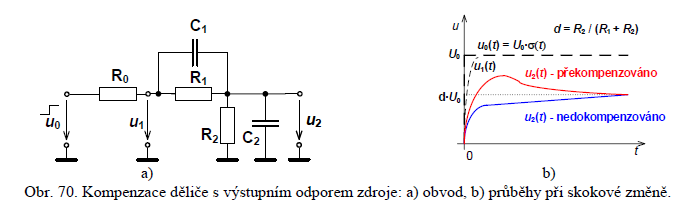
\includegraphics[width=0.7\linewidth]{Obrazky/AE2/2otazka/frekZavisDelicVystupnyOdpor}
	\caption{Kompenzácia deliča s výstupným odporom zdroja signálu}
	\label{fig:frekzavisdelicvystupnyodpor}
\end{figure}
\section{Diódové funkčne meniče}
Jedná sa o nelineárne obvody určené na tvarovanie či orezávanie signálu v časovej oblasti. Využíva sa vedenie prúdu diódou len jedným smerom. 
\subsection{Diódový obmedzovač}
\begin{itemize}
	\item Delič napätia s nelineárnym prvkom
	\item Minimálna hodnota napätia je daná PN prechodom diódy $\rightarrow$ cca \qty{0.6}{\V} čo môže byť problém
	\item V prípade, že chceme obmedziť vyššie napätie ako je \qty{0.6}{\V} môžeme to urobiť pridaním zdroja napätia sériovo s diódou $\rightarrow$ efektívne sa posunie hranica orezávania o hodnotu priloženého napätia.
	\subitem Zdroj napätia vieme riešiť napríklad buffrom, ktorý má \emph{umelú zem}
\end{itemize}
\begin{figure}[H]
	\centering
	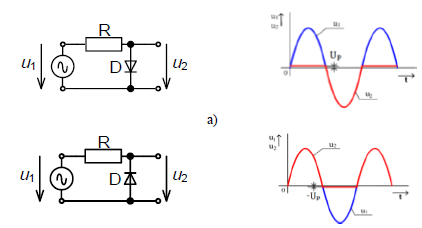
\includegraphics[width=0.7\linewidth]{Obrazky/AE2/2otazka/diodovyObmedzovac}
	\caption{Príklad diódového obmedzovača}
	\label{fig:diodovyobmedzovac}
\end{figure}
\begin{figure}[H]
	\centering
	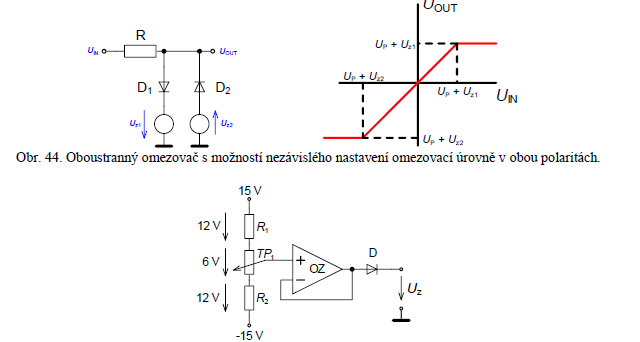
\includegraphics[width=0.7\linewidth]{Obrazky/AE2/2otazka/diodovyObmedzovacObojsmerny}
	\caption{Obojsmerný diódový obmedzovač}
	\label{fig:diodovyobmedzovacobojsmerny}
\end{figure}
\subsection{Diódový vykrajovač}
\begin{itemize}
	\item Úlohou je vykrojiť len časť priebehu.
	\item Nesleduje sa napätie ale sleduje sa prúd pretekajúci diódou.
	\item Znovu je možné stanoviť hodnoty vykrajovania pre obe polarity vstupného napätia.
	\item Strmosť výstupnej charakteristiky je daná odporom $R_5$
	\item Z princípu je výstupný signál invertovaný
\end{itemize}
\begin{figure}[H]
	\centering
	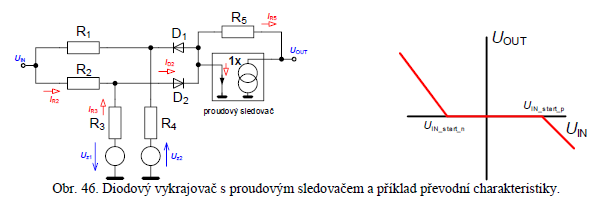
\includegraphics[width=0.7\linewidth]{Obrazky/AE2/2otazka/diodovyVykrajovac}
	\caption{Ukážka diódového vykrajovača}
	\label{fig:diodovyvykrajovac}
\end{figure}
\subsection{Diódový tvarovač}
\begin{itemize}
	\item Jedná sa o funkčný meniť.
	\item Používa sa pre aproximáciu harmonického signálu $\rightarrow$ metódou lomených priamok.
	\item Spracováva pílový vstupný signál, pričom frekvencia je obmedzená len parazitnými kapacitami obvodu.
	\item Nesmie sa meniť vstupná amplitúda signálu.
	\item Môže byť nepraktické pre malé signály.
	\item Polperiódu signálu je nutné rozdeliť na nepárny počet úsekov $\rightarrow$ inak by vznikla v maxime ostrá špička $\rightarrow$ počet úsekov je rovný počtu segmentov diódového tvarovača.
	\item Jedná sa znovu o odporový delič, pričom jeho odpory sa menia podľa otvárania diód $\rightarrow$ mení sa strmosť výstupu.
	\item Vzdialenosti medzi úsekmi sa dajú aproximovať rôzne, napríklad ekvidistantnou vzdialenosťou medzi hranicami.
\end{itemize}
\begin{figure}[H]
	\centering
	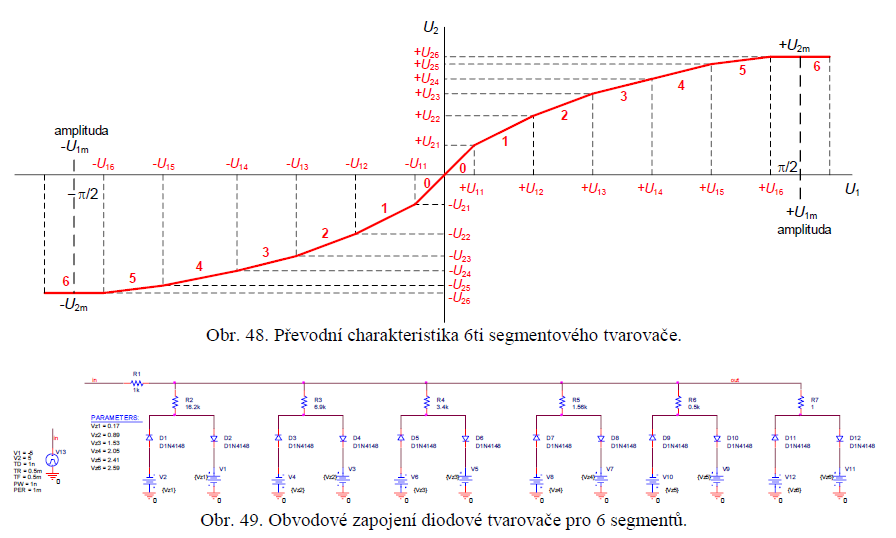
\includegraphics[width=0.9\linewidth]{Obrazky/AE2/2otazka/diodovyTvarovac}
	\caption{Ukážka prevodnej charakteristiky a zapojenia šesť segmentového diódového tvarovača.}
	\label{fig:diodovytvarovac}
\end{figure}
\section{Bipolárny tranzistorový spínač}
\begin{itemize}
	\item Návrh podstatne zložitejší ako pri Unipolárnych spínačoch
	\item Pri návrhu sa nedajú aplikovať malosignálové úvahy
	\item Na návrh jedného stupňa stačí v podstate len bázový odpor, ktorý nastaví potrebný prúd do báze, pre dosiahnutie požadovaného prúdového zosilnenia
	\item Viacstupňový návrh je v podstate dynamické spínanie odporových deličov, kedy jeden stupeň spína odporový delič na svojom výstupe a tým nastavuje pracovné podmienky pre spustenie ďalšieho stupňa.
	\item Celý návrh je v podstate len odhad, nakoľko sa robí podstatne zjednodušený.
	\item Pri návrhu sa nedá uvažovať konštantný parameter $\beta$ $\rightarrow$ teda prúdový zosilovací činiteľ, nakoľko je závislý od kolektorového prúdu a teploty tranzistora.
	\subitem Navyše majú výkonové spínacie prvky podstatne nižšie hodnoty tohto činiteľa.
	\item Stručný postup návrhu:
	\begin{enumerate}
		\item Začína sa od konca $\rightarrow$ od záťaže, kedy na základe potrebného spínaného prúdu zistíme potrebný bázový prúd
		\item Pokračuje sa výpočtom deliča na vstupe posledného stupňa.
		\item Výpočet deliča závisí na prúde kolektorom predchádzajúceho stupňa
		\subitem a takto sa to točí xD :kappa: :vutEz:
	\end{enumerate}
	\item V procese návrhu je nutné využívať antisaturačné diódy, zapojené medzi bázu a kolektor.
	\subitem Ich úlohou je zaistiť aby nekleslo kolektorové napätie pod bázové napätie $\rightarrow$ dochádza k hlbokej saturácií.
	\subitem Dióda urýchľuje dobu spínania, no zvyšuje parazitnú kapacitu medzi C-B.
	\subitem Používajú sa Schottkyho diódy.
	\item Tento návrh má aj iné problémy:
	\subitem Saturačný úbytok napätia $\rightarrow$ pri veľkých prúdoch sa to bude hriať jak prasa na ražni
	\subitem Prúd do báze môže neprimerane zaťažovať riadiaci obvod
\end{itemize}
\begin{figure}[H]
	\begin{subfigure}[b]{0.48\textwidth}
		\centering
		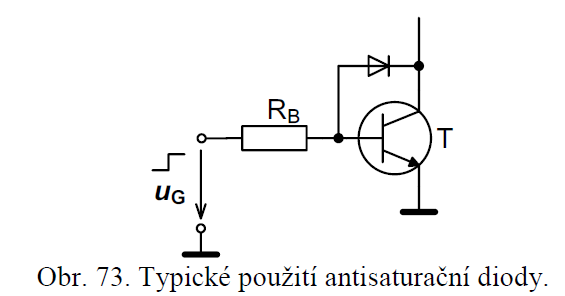
\includegraphics[width=0.7\linewidth]{Obrazky/AE2/2otazka/anitsaturacnaDioda}
		\caption{Príklad zapojenia antisaturačnej diódy}
		\label{fig:anitsaturacnadioda}
	\end{subfigure}
	\begin{subfigure}[b]{0.48\textwidth}
		\centering
		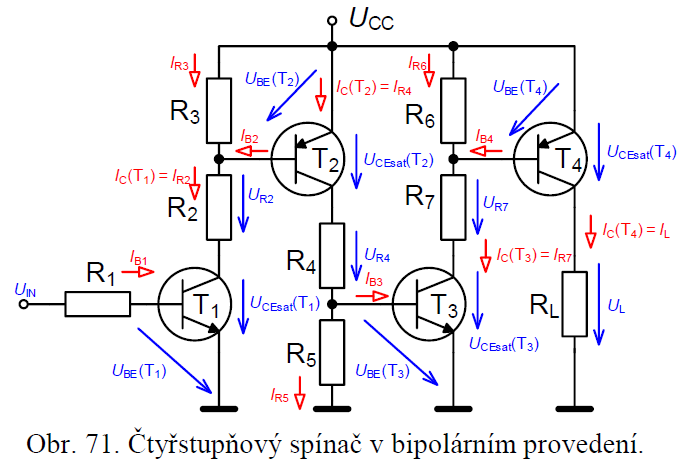
\includegraphics[width=0.7\linewidth]{Obrazky/AE2/2otazka/stvorstupnovySpicna}
		\caption{Príklad zapojenia štvorstupňového bipolárneho spínača}
		\label{fig:stvorstupnovyspicna}
	\end{subfigure}
\end{figure}
\section{Unipolárny tranzistorový spínač}
\begin{itemize}
	\item Jednoduché na návrh.
	\item Netrpí neduhmi bipolárnej štruktúry - menšie straty vďaka nízkemu odporu kanálu.
	\item Na druhú stranu majú výkonové unipolárne prvky majú vysokú kapacitu medzi G-S.
	\item Vysoká kapacita G-S znamená, že v okamihu vypnutia sú potrebné vysoké prúdy pre vybitie tejto kapacity
	\item Častokrát sa používajú takzvané Drivers
	\begin{itemize}
		\item Úloha Driver-u je jasná $\rightarrow$ urýchliť spínanie a odpínanie MOS.
	\end{itemize}
	\item V podstate je všetko EZ a pohodka
\end{itemize}
\begin{figure}[H]
	\centering
	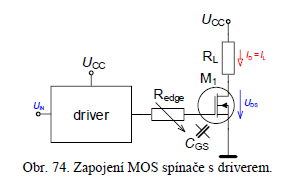
\includegraphics[width=0.5\linewidth]{Obrazky/AE2/2otazka/mosfetSpinac}
	\caption{Príklad zapojenia MOSFET spínača.}
	\label{fig:mosfetspinac}
\end{figure}
\section{Zdroje zákmitov}
\begin{itemize}
	\item Rýchle spínanie vyvoláva rezonančné zákmity $\rightarrow$ spôsobené parazitnou indukčnosťou a kapacitou v obvode $\rightarrow$ od stoviek kHz
	\item Pri veľkých záťažiach je to len viac problematické, je problém prekonať \qty{1}{\MHz}
	\item Rezonančná frekvencia zákmitov je daná Tompsonovým vzťahom \(f_{rez} = \frac{1}{2\pi \sqrt{L_p C_p}}\)
	\item Proti zákmitom sa dá bojovať s využitím \emph{Snubberu}, čo je paralelný RC obvod, pripojený k spínaciemu prvku
	\subitem Jeho princíp využíva vzájomné predávanie energie medzi cievkou a kondenzátorom
\end{itemize}
\begin{figure}[H]
	\centering
	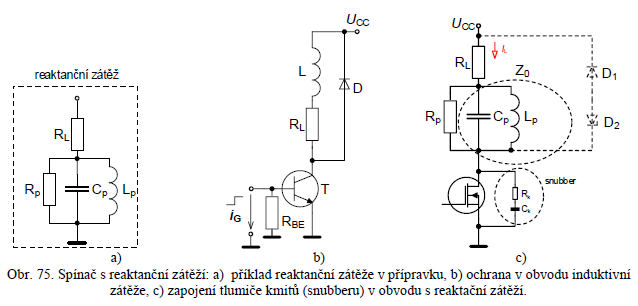
\includegraphics[width=0.7\linewidth]{Obrazky/AE2/2otazka/zdrojeZakmitov}
	\caption{Reaktančná záťaž a obrany voči zákmitom}
	\label{fig:zdrojezakmitov}
\end{figure}
Princíp návrhu \emph{snubberu}: (Písalo to AI)
\begin{itemize}
	\item \textbf{Hodnota rezistora $R_k$:} Musí sa pohybovať okolo charakteristickej impedancie obvodu, teda $R_k \le Z_0 = \sqrt{L_p/C_p}$, prípadne podľa zjednodušeného odhadu $R_k \le U_{CC}/I_L$.
	\item \textbf{Dimenzovanie rezistora $R_k$:} Musí byť schopný odolať špičkovému napätiu zodpovedajúcemu $U_{CC}$ v rozopnutom stave (OFF) a špičkovému prúdu zodpovedajúcemu prevádzkovému prúdu v zopnutom stave (ON).
	\item \textbf{Minimálna kapacita $C_k$:} Energia uložená v kondenzátore musí byť väčšia ako energia indukčnosti obvodu, z čoho vyplýva podmienka $C_{kmin} > L_p \cdot I_L^2 / U_{CC}^2$.
	\item \textbf{Časová konštanta obvodu:} Časová konštanta snubbra musí byť menšia ako desatina doby aktívneho stavu spínača, teda $R_k \cdot C_{kmax} < t_{on}/10$.
	\item \textbf{Celkový rozsah kapacity $C_k$:} Kapacita kondenzátora musí spĺňať výsledné operatívne rozmedzie: $\frac{L_p \cdot I_L^2}{U_{CC}^2} < C_k < \frac{t_{on}}{10}$.
	\item \textbf{Ochrana pri spínaní induktívnej záťaže:} Je nutné paralelne k záťaži pripojiť výkonovú diódu (prípadne v kombinácii so Zenerovou diódou), ktorá zamedzí prekmitom napätia nad úroveň $U_{CC}$ a ochráni spínač pred prekročením maximálnej straty.
	\item \textbf{Dimenzovanie ochranných diód:} Špičky prúdu tečúceho ochrannými diódami nesmú prekročiť ich maximálny povolený stratový príkon, inak je potrebné použiť zrážací odpor alebo zvoliť robustnejší typ diód.
\end{itemize}
\section{Výkonové straty pri spínaní}
\begin{itemize}
	\item  Straty na bipolárnej štruktúre:
	\begin{itemize}
		\item rozdeľujú sa na vstupné a výstupné
		\item vstupné
		\begin{itemize}
			\item Bázové straty - väčšinou zanedbateľné, kým bázou netečú veľké prúdy
		\end{itemize}
		\item výstupné
		\begin{itemize}
			\item statické (pri stabilnom stave zopnutého tranzistora)
			\subitem Jedná sa o súčin saturačného napätia tranzistora a prúdu kolektorom.
			\item dynamické (pri pravidelnom spínaní)
			\subitem napätia a prúdy v okamihu zopnutia či rozopnutia narastajú / klesajú exponencionálne
		\end{itemize}
	\end{itemize}
	\item  Straty na unipolárnej štruktúre:
	\begin{itemize}
		\item Vďaka malému odporu kanálu sú straty mizivé (pri nízkych prúdoch)
		\item Statické straty sa riadia podobne ako pri BJT
		\item Dynamické straty sú tiež podobné
	\end{itemize}
\end{itemize}
\section{Klopné obvody}
Rozlišujú dva typy stavov $\rightarrow$ stabilný a nestabilný stav. Prechod medzi stabilnými stavmi sa nazýva nestabilný stav. Základom klopných obvodov sú zosilňovače s kladnou spätnou väzbou. To sa dá realizovať tranzistorovými stupňami, minimálne dva. Podľa charakteru stabilných stavov rozlišujeme:
\begin{itemize}
	\item Bistabilný KO - oba stavy sú trvalo stabilné.
	\item Monostabilný KO - jeden stav je trvalo a druhý je dočasne stabilný.
	\item Astabilný KO - oba stavy sú dočasne stabilné, obvod nimi prechádza dookola.
	\item Dá sa realizovať z tranzistorov, z NOR hradiel, rovnako aj RS-KO obvod (pri vylúčení možnosti aktivácie R a S vstupov naraz)
\end{itemize}

\subsection{Bistabilný klopný obvod}
\begin{itemize}
	\item Pozostáva z dvoch tranzistorových stupňov s DC väzbou.
	\item Na zmenu stavu je potrebný vonkajší vstup.
	\item Tvoria základ pre registry, čítače a podobne.
\end{itemize}
\begin{figure}[H]
	\centering
	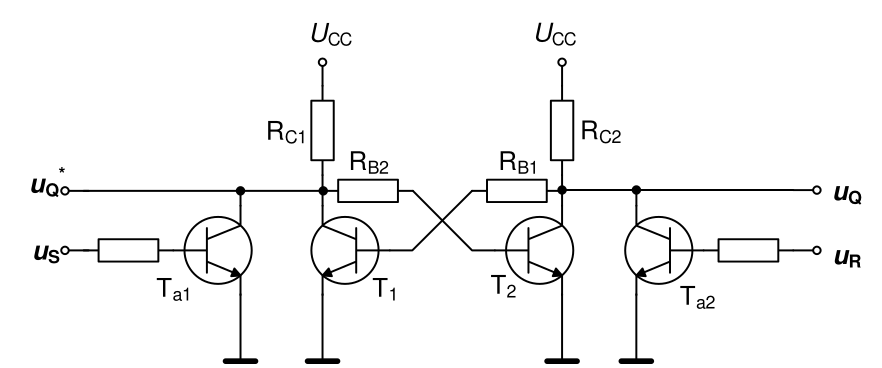
\includegraphics[width=0.7\linewidth]{Obrazky/AE2/2otazka/bkotrans}
	\caption{Bistabilný klopný obvod z tranzistorov}
	\label{fig:bkotrans}
\end{figure}
\begin{figure}[H]
	\centering
	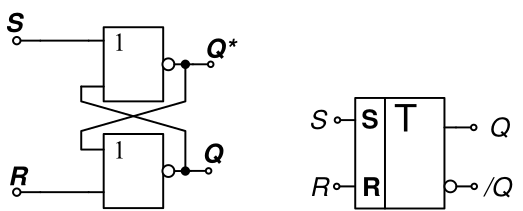
\includegraphics[width=0.45\linewidth]{Obrazky/AE2/2otazka/bkoLogi}
	\caption{Realizácia Bistrabilného klopného obvodu z NOR hradiel a RS-KO}
	\label{fig:bkologi}
\end{figure}
\subsection{Monostabilný klopný obvod}
\begin{itemize}
	\item Zapojenie vychádza zo zapojenia BKO, jedna spätná väzba je viazaná kondenzátorom.
	\item Po privedení napájacieho napätia je T2 otvorené T1 uzavreté. Kondenzátor C je nabitý na $U{CC}-U_{BE_{satT2}}$
	\item Spúšťací impulz skratne kolektor T1, spustí sa prebíjanie kondenzátora, T2 ostane uzavretý do doby kým sa napätie na C nevráti na pôvodnú úroveň.
	\item Časová konštanta $\tau = R_{B2} C$
	\item Doba zotavenia $t_i = \ln(2)\tau$
	\item Klasické MKO reaguje na spúšťací impulz len pokiaľ je v stabilnom stave.
	\item Existujú aj znovu spustiteľné MKO, ktoré zakaždým resetujú dobu zotavenia.
	\item Je možná realizácia aj s 555 časovačom.
\end{itemize}
\begin{figure}[H]
	\centering
	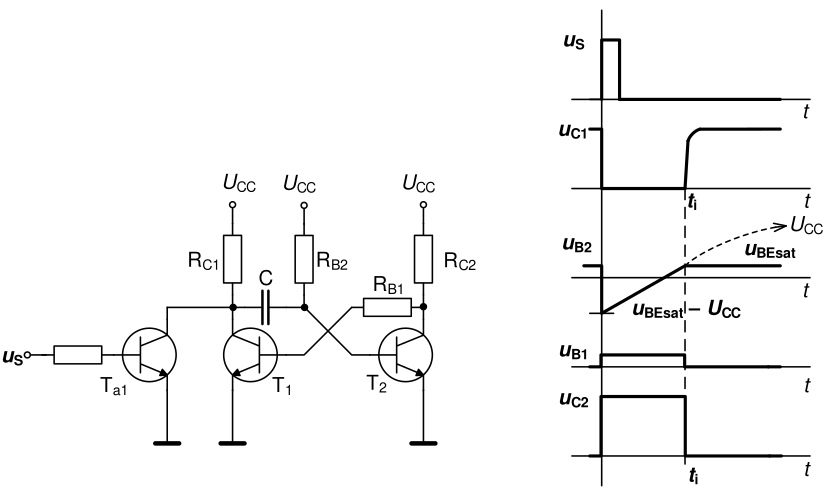
\includegraphics[width=0.55\linewidth]{Obrazky/AE2/2otazka/mkoTrans}
	\caption{Zapojenie MKO spolu s časovými pribehmi.}
	\label{fig:mkotrans}
\end{figure}
\begin{figure}[H]
	\centering
	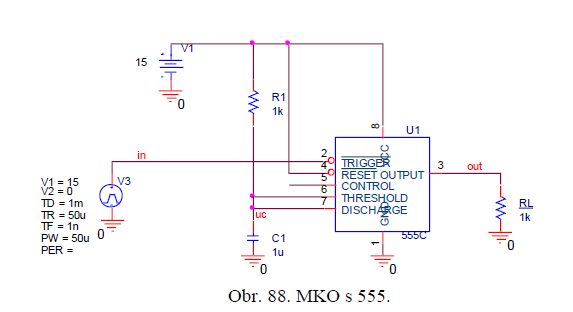
\includegraphics[width=0.7\linewidth]{Obrazky/AE2/2otazka/mko555}
	\caption{Realizácia MKO s časovačom 555, $t_i = \tau \ln(3)$}
	\label{fig:mko555}
\end{figure}
\subsection{Astabilný klopný obvod} 
\begin{itemize}
	\item Vychádzajú z MKO, kedy sú obe spätné väzby nahradené kondenzátorovou väzbou.
	\item Neustále sa preklápajú, nemajú spúšťací impulz, potrebujú len napájanie.
	\item Používajú sa na ľahké generovanie pravouhlých impulzov.
	\item V RF technike sa z nich po filtrácií dá generovať aj harmonický signál.
	\item Možná realizácia aj s časovačom 555.
	\item Nastavenie periódy je možné: 
	\item \[T = t_1 + t_2 = (R_{B1} C_1 + R_{B2} C_2) \ln(2) = \frac{1}{f_0}\]
\end{itemize}
\begin{figure}[H]
	\centering
	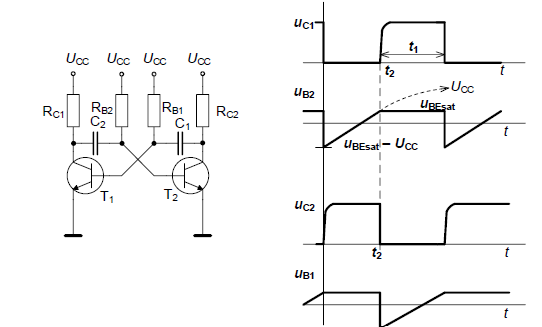
\includegraphics[width=0.55\linewidth]{Obrazky/AE2/2otazka/akoTrans}
	\caption{Zapojenie AKO spolu s časovými priebehmi.}
	\label{fig:akotrans}
\end{figure}
\begin{figure}[H]
	\centering
	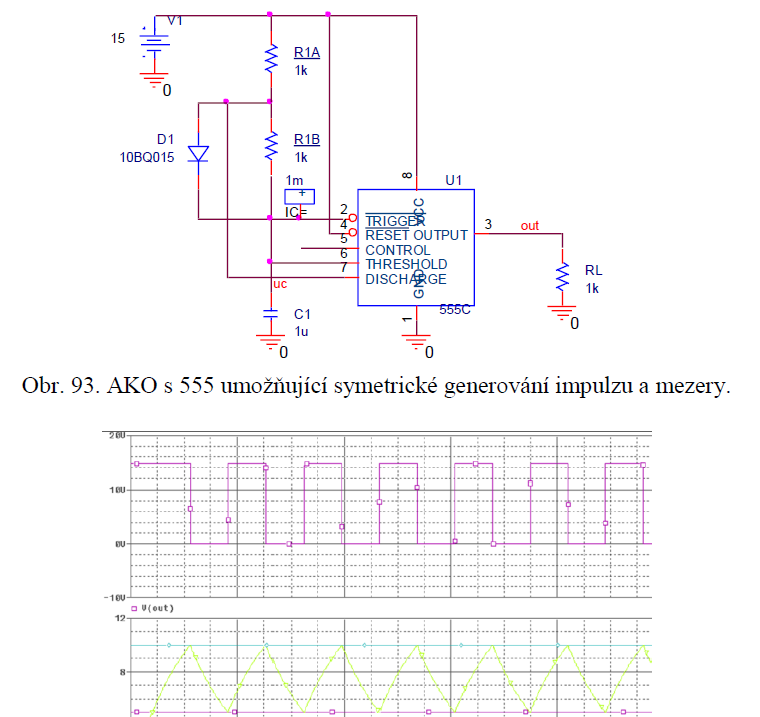
\includegraphics[width=0.7\linewidth]{Obrazky/AE2/2otazka/ako555}
	\caption{AKO s časovačom 555}
	\label{fig:ako555}
\end{figure}
\subsection{Klopné obvody s logických prvkov - hradiel}
Klopný obvod je možné realizovať s RS blokom, rovnako aj s radou TTL hradiel.
\section{Komparátory}
\subsection{Tranzistor ako invertujúci komparátor}
\begin{itemize}
	\item Najjednoduchší komparátor.
	\item Z povahy je invertujúceho charakteru.
	\item Rozhodovacia úroveň napätia je daná bázovým napätím tranzistora $\rightarrow$ \qty{0.7}{\V}.
	\item Užíva sa ochranná dióda, pre ochranu voči zápornému napätiu.
	\item Nehrozí rozkmitanie, vhodný pre veľké vstupné signály.
	\item Pokiaľ vstupné napätie prechádza oblasťou rozhodovacej úrovne pomaly $\rightarrow$ dochádza k spojitej zmene výstupného napätia.
\end{itemize}
\begin{figure}[H]
	\centering
	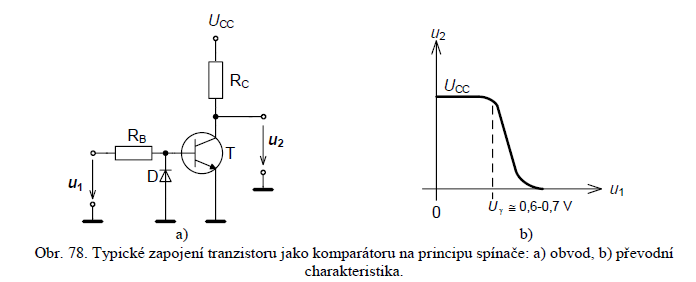
\includegraphics[width=0.55\linewidth]{Obrazky/AE2/2otazka/tranzistorInvertKomp}
	\caption{Invertujúci tranzistorový komparátor.}
	\label{fig:tranzistorinvertkomp}
\end{figure}
\subsection{Tranzistor ako neinvertujúci komparátor}
\begin{itemize}
	\item Vychádza z invertujúceho zapojenia $\rightarrow$ prosté zapojenie jednotlivých stupňov do kaskády.
	\item Dvojité zapojenie invertujúcich stupňov odstráni inverziu.
	\item Dosahuje sa vyššej úrovne zosilnenia výstupu.
	\item Nebezpečenstvo rozkmitania.
	\subitem Rozkmitanie sa dá potlačiť kladnou spätnou väzbou.
	\item KZV nám vytvorí v obvode hysterézu.
	\item S hysterézou sú zmeny napätia skokové.
	\item Nepoužívajú sa často $\rightarrow$ nemožnosť nastavenia rozhodovacej úrovne $\rightarrow$ nahradené Schmittovým komparátorom.
	\item Teplotne závislé.
\end{itemize}
\begin{figure}[H]
	\centering
	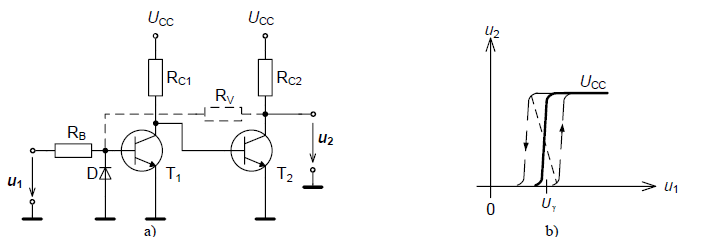
\includegraphics[width=0.55\linewidth]{Obrazky/AE2/2otazka/neinvertujuciKomparatorTrans}
	\caption{Zapojenie neinvertujúceho tranzistorového komparátora.}
	\label{fig:neinvertujucikomparatortrans}
\end{figure}
\subsection{Komparátor s diferenčným vstupom}
\begin{itemize}
	\item Zníženie teplotnej závislosti.
	\item V základnej podobe nevie robiť menej ako \qty{0.5}{\V}. Ak chceme nižšiu hodnotu potrebujeme symetrické napájanie.
	\item Nazýva sa komparačný zosilňovač.
\end{itemize}
\begin{figure}[H]
	\centering
	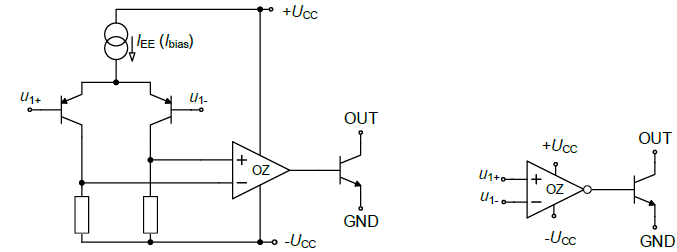
\includegraphics[width=0.55\linewidth]{Obrazky/AE2/2otazka/diferencnyKomparator}
	\caption{Typický komparátor s diferenciálnym vstupom}
	\label{fig:diferencnykomparator}
\end{figure}
\subsection{Zapojenie komparátora s komparačným zosilňovačom}
\begin{itemize}
	\item K zmene výstupu dochádza pri rovnosti vstupného napätia.
	\item Komparačné úrovne sú dané hodnotami rezistorov.
	\item Rozhodovacia úroveň je závislá na veľkosti záťaže $\rightarrow$ toto môže byť problém.
	\item Bežne sa realizujú s výstupom typu \emph{otvorený kolektor $\rightarrow$ open drain}.
	\item Má invertujúci charakter $\rightarrow$ dá sa vytvoriť aj neinvertujúci, ak sa vytvorí delič na neinvertujúcom vstupe a zavedie spätná väzba podobne ako pri dvojstupňovom tranzistorovom komparátore.
\end{itemize}
\begin{figure}[H]
	\centering
	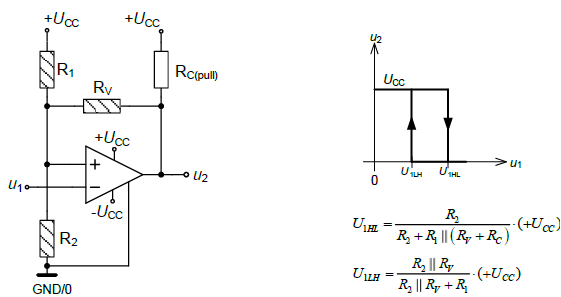
\includegraphics[width=0.55\linewidth]{Obrazky/AE2/2otazka/komparator}
	\caption{Zapojenie komparačného zosilňovača.}
	\label{fig:komparator}
\end{figure}
\section{Zapojenie OZ ako komparátora}
\begin{itemize}
	\item Klasické OZ nie sú určené na prácu v saturačnom režime.
	\item Pri návrate z nasýtenia do lineárnej oblasti sa prajavuje saturačné oneskorenie výstupu.
	\item OZ sa nehodia používať tam kde je potrebná rýchla odozva.
	\item Výhoda tohto je aj dvojčinné zapojenie výstupu, spínač na zápornú aj kladnú svorku.
	\item Výstupné napätie v saturácií sa lýši od napájacieho napätia $\rightarrow$ lepšie použiť Rail-To-Rail.
	\item Nepresnosť výstupného napätia je ovplyvnená teplotou.
\end{itemize}
\begin{figure}[H]
	\centering
	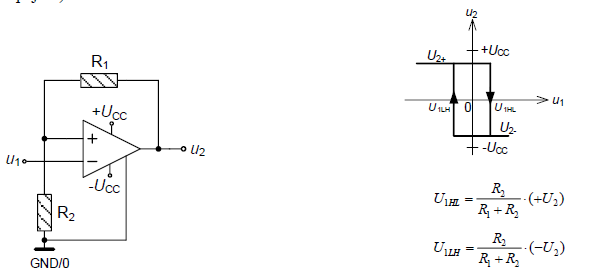
\includegraphics[width=0.7\linewidth]{Obrazky/AE2/2otazka/komparatorOZ}
	\caption{Zapojenie klasického OZ ako komparátora.}
	\label{fig:komparatoroz}
\end{figure}
\subsection{Okienkový komparátor}
\begin{itemize}
	\item Dvojica komparátorov s jednou rozhodovacou úrovňou, výstup viazaný logickým blokom.
	\item Sú potrebné dve referenčné napätia.
	\item Neivertujúce zapojenie.
	\item Rozhodovacie úrovne dané referenčným napätím, nie záťažou.
	\item Presný komparátor s hysterézou.
	\item Pri modifikácií s RS-KO je možné dosiahnuť hysterézu.
	\item Časovač 555 JE okienkový komparátor.
\end{itemize}
\begin{figure}[H]
	\centering
	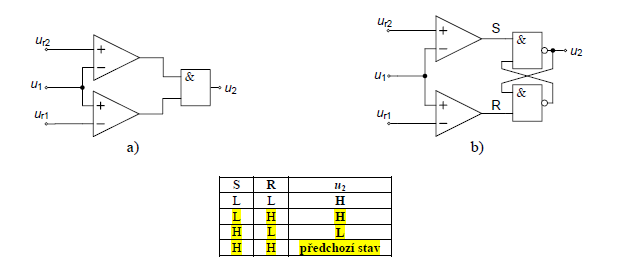
\includegraphics[width=0.7\linewidth]{Obrazky/AE2/2otazka/okienkovyKomparatro}
	\caption{Okienkový komparátor a jeho modifikácia s RS-KO}
	\label{fig:okienkovykomparatro}
\end{figure}
\begin{figure}[H]
	\centering
	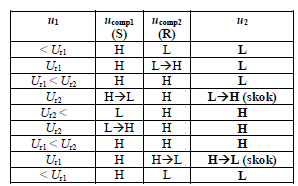
\includegraphics[width=0.7\linewidth]{Obrazky/AE2/2otazka/RSKOkomparatorStavy}
	\caption{Tabuľka stavov komparátora s RS-KO}
	\label{fig:rskokomparatorstavy}
\end{figure}
\section{Generátory priebehov}
\subsection{Relaxačný generátor $\rightarrow$ multivibrátor}
\begin{itemize}
	\item Základný blok je integračný RC článok a OZ.
	\item Komparátor musí byť invertujúcej povahy.
	\item Dosiahnutie komparačnej úrovne na vstupe vyvolá zmenu výstupu, teda ak sa kondík nabíjal, tak sa začne vybíjať.
	\item Komparačná úroveň je nastavená referenčným napätím na deliči pripojenom na neinvertujúci vstup.
	\item Po štarte obvodu je čas preklopenia výstupu $t_1$ iný ako čas po ustálení obvodu.
	\item Celá perióda opakovania je vyjadrená:
	\begin{equation}
		T = \frac{1}{f_0} = 2 R C \ln\left(\frac{R_a + 2 R_b}{R_a}\right)
	\end{equation}
	\item Vyžaduje sa symetrické napájanie $\rightarrow$ dve porovnávacie úrovne $\rightarrow$ $U_{Ref2} = -U_{Ref1}$
	\item Vyhovuje použiť Rail-To-Rail operák.
	\item Možnosť zmeny striedy výstupného signálu je ak $R_b$ neuzemníme ale posadíme ho na DC zdroj.
\end{itemize}

\begin{figure}[H]
	\begin{subfigure}[b]{0.48\textwidth}
		\centering
		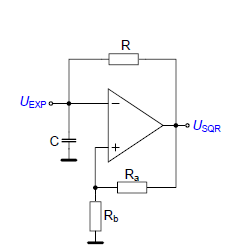
\includegraphics{Obrazky/AE2/2otazka/multivibratorZapojenie}	
		\caption{Zapojenie multivibrátora.}
		\label{fig:multivibratorzapojenie}
	\end{subfigure}
	\begin{subfigure}[b]{0.48\textwidth}
		\centering
		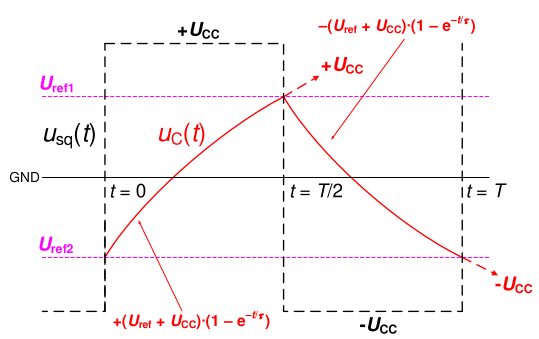
\includegraphics[width=0.7\linewidth]{Obrazky/AE2/2otazka/multivibratorPriebehy}
		\caption{Priebeh napätia v uzloch multivibrátora}
		\label{fig:multivibratorpriebehy}
	\end{subfigure}
\end{figure}
\subsection{Funkčný generátor s bezstratovým integrátorom}
\begin{itemize}
	\item Nahrádza stratový integračný článok bezstratovým integrátorom. $\rightarrow$ Kondík sa nabíja konštantným prúdom $\rightarrow$ výsledok je lineárny nárast napätia na kondenzátore.
	\item Umožňuje získať pílový alebo trojuholníkový priebeh.
	\item Vychádza z relaxačného generátoru, pridáva sa buď invertujúci jednotkový zosilňovač alebo neinvertujúci komparátor.
	\item Je potrebný invertujúci integrátor.
\end{itemize}
\begin{figure}[H]
	\centering
	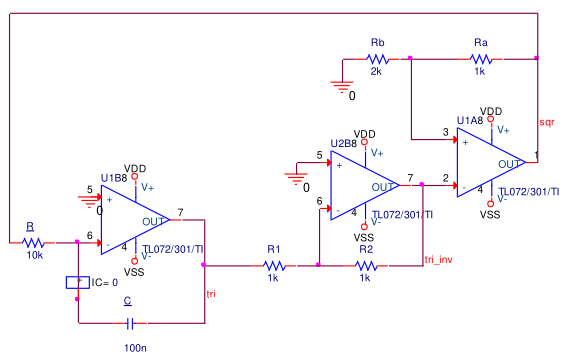
\includegraphics[width=0.45\linewidth]{Obrazky/AE2/2otazka/funkcnyGeneratorZapojenie2}
	\caption{Zapojenie funkčného generátora, s invertujúcim komparátorom}
	\label{fig:funkcnygeneratorzapojenie2}
\end{figure}
\begin{equation}
	T = \frac{1}{f_0} = 4 R C \left(\frac{R_b}{R_a + R_b}\right)
\end{equation}
\begin{figure}[H]
	\begin{subfigure}[b]{0.48\textwidth}
		\centering
		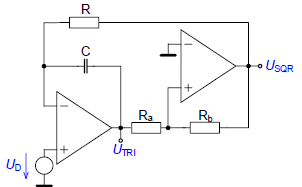
\includegraphics[width=0.7\linewidth]{Obrazky/AE2/2otazka/funkcnyGeneratorZapojenie}
		\caption{Zapojenie funkčného generátora.}
		\label{fig:funkcnygeneratorzapojenie}
	\end{subfigure}
	\begin{subfigure}[b]{0.48\textwidth}
		\centering
		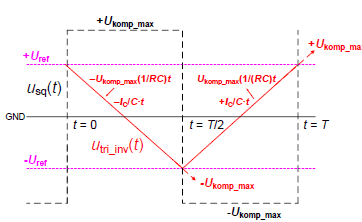
\includegraphics[width=0.7\linewidth]{Obrazky/AE2/2otazka/funkcnyGeneratorPriebehy}
		\caption{Priebehy funkčného generátora s neinvertujúcim komparátorom.}
		\label{fig:funkcnygeneratorpriebehy}
	\end{subfigure}
	\caption{Funkčný generátor s neinvertujúcim komparátorom}
	\label{fig:gen}
\end{figure}
\begin{equation}
	T = \frac{1}{f_0} = 4 R C \left(\frac{R_a}{R_b}\right)
\end{equation}
Pre zapojenie \ref{fig:gen} je možné meniť striedu generátora DC zdrojom napätia. Rovnako je možné využiť iné spôsoby:
\begin{figure}[H]
	\centering
	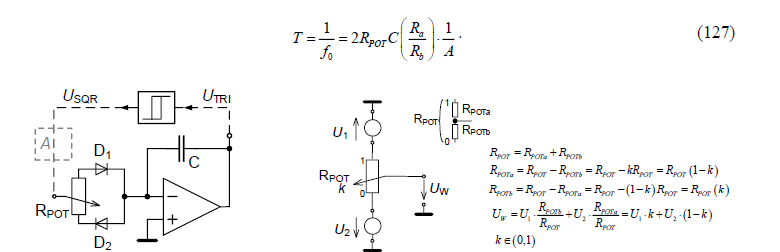
\includegraphics[width=0.8\linewidth]{Obrazky/AE2/2otazka/riadenieGeneratora}
	\caption{Riadenie Striedy a Frekvencie generátora.}
	\label{fig:riadeniegeneratora}
\end{figure}
\begin{itemize}
	\item Strieda sa riadi pomocou potenciometra.
	\item Frekvencia sa riadi pomocou vloženého lineárneho zosilňovača
\end{itemize}
\subsection{Generátor s 555}
\begin{figure}[H]
	\centering
	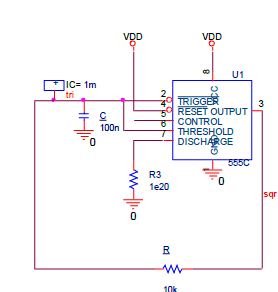
\includegraphics[width=0.35\linewidth]{Obrazky/AE2/2otazka/generator555}
	\caption{Funkčný generátor s časovačom 555 $\rightarrow$ nie je to AKO}
	\label{fig:generator555}
\end{figure}
\begin{itemize}
	\item 555 samé o sebe nedokáže urobiť \qty{50}{\%} striedu
	\item Komparátor je realizovaný spôsobom, kedy je C nabíjané z 555, nie z $U_{CC}$
	\item Využíva sa interného okienkového komparátoru 555.
	\item Oproti AKO sa ušetrí jedna dióda a odpor.
	\item \[T = 2 R C \ln(2)\]
\end{itemize}
\subsection{Generátor s CCII+}
\begin{itemize}
	\item Prúdový konvejor
	\item Využíva sa internej väzby pre komparátor (prúd záporného vstupu = prúd prúdového výstupu)
\end{itemize}
\begin{figure}[H]
	\centering
	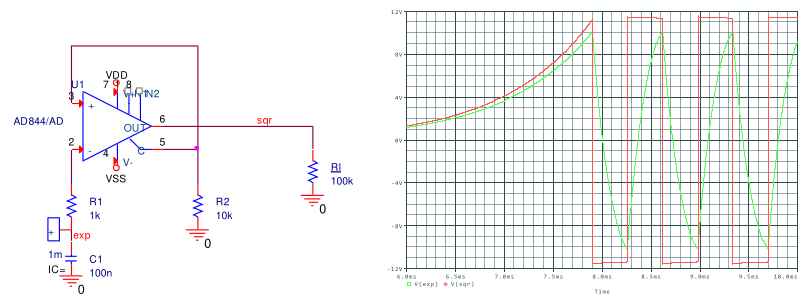
\includegraphics[width=0.7\linewidth]{Obrazky/AE2/2otazka/CCIIgen}
	\caption{Generátor s CCII+ - AD844}
	\label{fig:cciigen}
\end{figure}

\subsection{Generátor OTA}
\begin{itemize}
	\item Jednoduchá aplikácia.
	\item Úsporné riešenie, jedno z najlepších.
	\item Ľahká realizácia bezstratového integrátora, či už invertujúceho alebo neinvertujúceho.
	\item Komparačné hladiny sú $\pm$ maximálne napätie na $R$ v komparátore. Toto sa dá upraviť deličom.
	\subitem Komparátor funguje tak, že pri prebudení OTA, je na výstupe maximálny možný prúd s danou polaritou.
	\item Výhoda je zemnená kapacita.
	\item Dá sa modifikovať tak, že sa to celé riadi zdrojom prúdu.
	\item Bežné moderné riešenie na čipe.
	\item Možnosť zmeny frekvencie aj striedy nezávisle na sebe.
	\item Strieda sa dá ovplyvniť len pridaním zdroja prúdu ku kondenzátoru.
\end{itemize}
\begin{figure}[H]
	\centering
	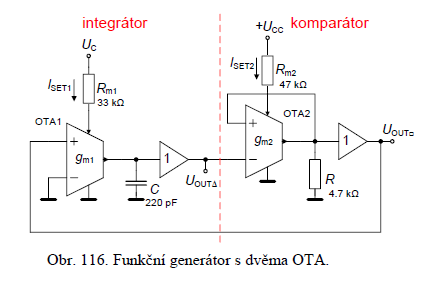
\includegraphics[width=0.7\linewidth]{Obrazky/AE2/2otazka/generatorOTA}
	\caption{Generátor postavený z OTA}
	\label{fig:generatorota}
\end{figure}

\chapter{Operačné zosilňovače, vlastnosti a použitie}
\section{Kmitočtové charakteristiky OZ}
Operačný zosilňovač so spätnou väzbou je uzavretý systém, ktorý je popísaný Blackovým vzťahom $\rightarrow$ teda môže dochádzať k nestabilite. Stabilitu OZ vieme vyšetriť na základe Nyquistovho či Bodeho kritéria stability.
\subsection{Nyquistovo kritérium stability}
\begin{itemize}
	\item Hodograf
	\item Závislosť imaginárnej zložky prenosu $\beta(j\omega)A(j\omega)$ na reálnej zložke.
	\item Systém je stabilný pokiaľ krivka v komplexnej rovine neobopína a ani neprechádza bodom $\left[1,0j\right]$
\end{itemize}
\begin{figure}[H]
	\centering
	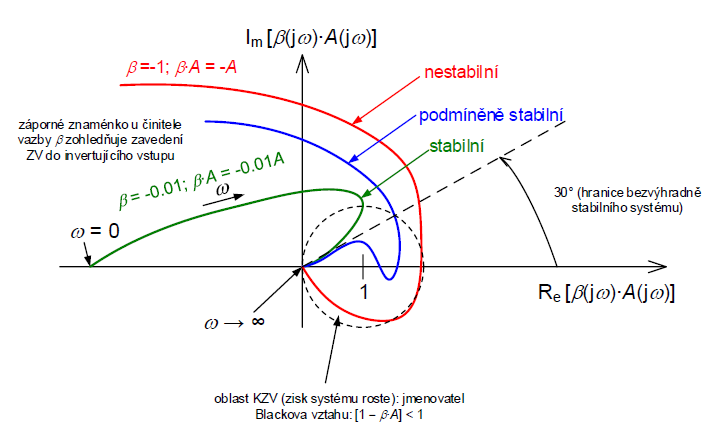
\includegraphics[width=0.7\linewidth]{Obrazky/AE2/3otazka/hodografNyquist}
	\caption{Komplexné zobrazenie Nyquistovej podmienky stability.}
	\label{fig:hodografnyquist}
\end{figure}
\subsection{Bodeho kritérium stability - GM, PM}
Zaoberá sa fázovou a amplitúdovou rezervou ktorá chýba v otvorenej slučke k dosiahnutiu zisku 1 a fázového posuvu \qty{-180}{\degree} $\rightarrow$ teda k dosiahnutiu nestabilného stavu.
\begin{itemize}
	\item Stabilný systém je ak má minimálne fázovú bezpečnosť $\text{PM} >= 45^\circ$
	\subitem V praxi sa zvykne vyžadovať $\text{PM} >= 60^\circ$ $\rightarrow$ zvýšená fázová bezpečnosť postihuje start-up stavy, impulzy a pod.
	\item Čím väčší je menovateľ Blackovho vzťahu $\rightarrow$ tým väčší je zisk systému $\rightarrow$ blíži sa k nestabilite.
	\item Jedno z Bodeho kritérií stability: Prenos celej slučky prechádza frekvenčnou osou v bode 0dB s maximálnym sklonom \qty{-40}{dB/dec} $\rightarrow$ teda ide maximálne o obvod 2. rádu.
	\item Najlepšie je ak sa frekvenčná os pretína so sklonom \qty{-20}{dB/dec}, nakoľko vtedy nedochádza k vzniku oblastí kladnej spätnej väzby a celková odozva je bez rezonančných prevýšení.
	\item \textbf{Bodeho poučka o stabilite:} Systém bude stabilný, ak je rozdiel strmostí charakteristík inverznej spätnej väzby $|1/\beta(j\omega)|$ a zisku zosilňovača $|A(j\omega)|$ v mieste priesečníku $20\text{ dB/dek}$ (najviac $40\text{ dB/dek}$ s dostatočnou rezervou pred ďalším zlomom).
\end{itemize}
\begin{figure}[H]
	\centering
	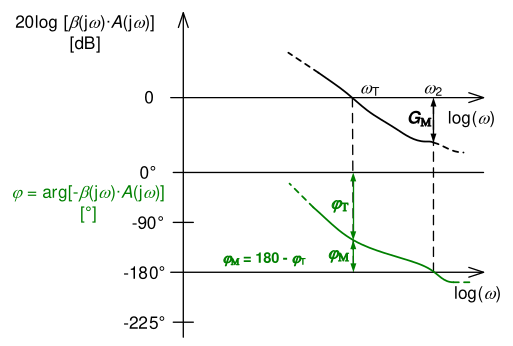
\includegraphics[width=0.6\linewidth]{Obrazky/AE2/3otazka/bodehoDiagram}
	\caption{Bodeho diagram}
	\label{fig:bodehodiagram}
\end{figure}
\begin{figure}[H]
	\centering
	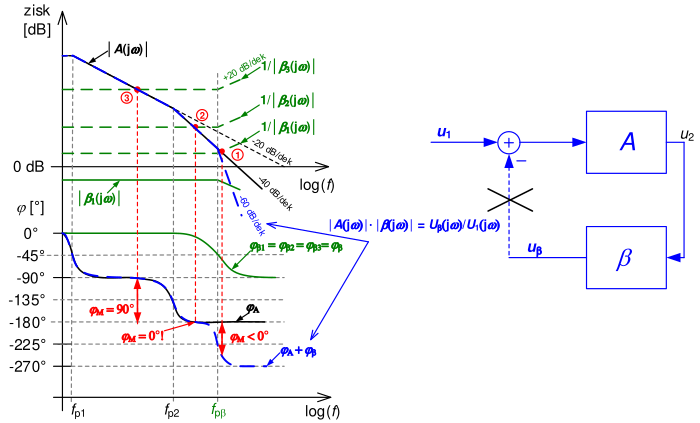
\includegraphics[width=0.7\linewidth]{Obrazky/AE2/3otazka/bodehoDiagramPopis}
	\caption{Frekvenčná charakteristika celého systému pri rozpojenej slučke, dielči prenos zosilňovača a spätnej väzby.}
	\label{fig:bodehodiagrampopis}
\end{figure}
\begin{description}
	\item[Bod č. 1:] Pretína sa tu frekvenčná závislosť $A(j\omega)$ a $\beta_1 (j\omega)$, ale fázová rezerva je menšia ako $0$, preto je obvod nestabilný. Energie a zisku je na to stále dosť (nad $0\text{ dB}$), no neprejaví sa to zrejme priamo osciláciami, ale skôr trvalou saturáciou výstupu, prípadne pri budení signálom preklápaním $\rightarrow$ v tomto stave ide vlastne o "komparátor", pretože má kladnú spätnú väzbu. Podmienka stability v bode č. 1 rozhodne nie je splnená, keďže rozdiel strmostí činí $|1/\beta_1(j\omega)| - |A(j\omega)| = +20\text{ dB/dek} - (-40\text{ dB/dek}) = +60\text{ dB/dek}$.
	
	\item[Bod č. 2:] Nachádzame sa presne na medzi stability (nulová fázová rezerva). Systém opäť pravdepodobne nebude kmitat harmonicky, ale bude v saturácii, pretože zosilnenie je pomerne vysoké. Pre harmonické kmitanie by pri splnení fázovej podmienky muselo byť zosilnenie nižšie, len mierne nad $0\text{ dB}$. Rozdiel strmostí modulov je teraz $+40\text{ dB/dek}$, ale je vidieť, že sa už nachádzame za ďalším zlomom ($f_{p2}$).
	
	\item[Bod č. 3:] Systém je stabilný, pretože fázová bezpečnosť je dostatočne väčšia ako $45^\circ$ a rozdiel strmostí modulov je $+20\text{ dB/dek}$.
\end{description}
\section{Kompenzácia frekvenčnej charakteristiky}
Frekvenčnú charakteristiku vieme kompenzovať:
\begin{itemize}
	\item Odstránením ďalších bodov zlomu $\rightarrow$ pólov nad \qty{0}{\dB}.
	\item Odstránenie zlomu z spätnej väzbe.
\end{itemize}
Popis korekcie:
\begin{itemize}
	\item \textbf{Cieľ korekcie:} Zabezpečiť, aby charakteristika zosilňovania klesala v mieste prechodu cez os $0\text{ dB}$ (jednotkový zisk) miernym sklonom – ideálne len $-20\text{ dB/dek}$ (maximálne $-40\text{ dB/dek}$), čo zaručuje stabilitu.
	
	\item \textbf{Vyrušenie kritického pólu (metóda pól-nula):} Korekčný obvod na vstupe vytvorí v charakteristike tzv. "nulu" ($\tau_a$), ktorú presne naladíme na frekvenciu prvého pólu zosilňovača ($\tau_1$). Táto nula kompletne vymaže (vyruší) pôvodný zlom zosilňovača, takže charakteristika v danom mieste nezačne padať strmšie.
	
	\item \textbf{Vytvorenie nového dominantného pólu:} Korekčný obvod namiesto toho zavedie nový, umelý pól na oveľa nižšej frekvencii ($f_b$). Zisk tak začne klesať oveľa skôr, no kontrolovane a pozvoľna.
	
	\item \textbf{Zníženie jednosmerného (DC) zisku:} Pomocou sériového odporu $R_S$ na vstupe sa zámerne o niečo zníži celkový zisk systému. Tým sa celá frekvenčná charakteristika posunie smerom nadol a tretí (nebezpečný) pól zosilňovača sa dostane bezpečne pod úroveň $0\text{ dB}$, kde už nemôže spôsobiť nestabilitu.
	
	\item \textbf{Alternatíva (Vnútorná kompenzácia):} Okrem externých súčiastok na vstupe (ako $R_k, C_k$) sa stabilita často rieši aj pripojením internej kompenzačnej kapacity priamo do vnútornej tranzistorovej štruktúry operačného zosilňovača.
\end{itemize}
\begin{figure}[H]
	\centering
	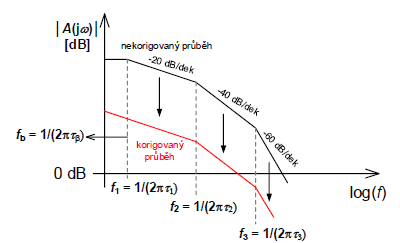
\includegraphics[width=0.55\linewidth]{Obrazky/AE2/3otazka/KorekciaFrekChar}
	\caption{Korekcia frekvenčnej charakteristiky zosilňovača $\rightarrow$ zníženie strmosti prechodu \qty{0}{\dB}.}
	\label{fig:korekciafrekchar}
\end{figure}
\begin{figure}[H]
	\begin{subfigure}[b]{0.48\textwidth}
		\centering
		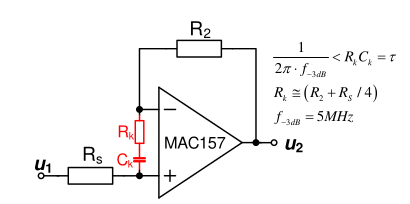
\includegraphics[width=0.7\linewidth]{Obrazky/AE2/3otazka/korekeciaPredOZ}
		\caption{Príklad korekcie pred vstupom do OZ}
		\label{fig:korekeciapredoz}
	\end{subfigure}
	\begin{subfigure}[b]{0.48\textwidth}
		\centering
		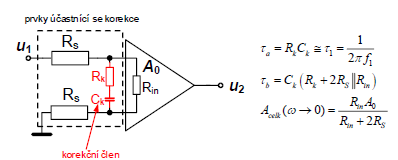
\includegraphics[width=0.7\linewidth]{Obrazky/AE2/3otazka/korekeciaVoVnutriOZ}
		\caption{Príklad korekcie priamo v OZ}
		\label{fig:korekeciavovnutrioz}
	\end{subfigure}
\end{figure}
\section{Kompenzácia kapacitnej záťaže OZ}
\begin{itemize}
	\item Zmiernenie vplyvu kapacitnej záťaže je možné úpravou spätnej väzby ZV.
	\item Parazitná kapacita na výstupe $\rightarrow$ teda aj kapacitná záťaž $\rightarrow$ vzniká kapacitami na DPS, pripojenými káblami BNC, hradlá unipolárov výkonových.
	\item Kapacitu je ťažké definovať, niektoré OZ s ňou počítajú do istej miery.
	\item Vplyvom kapacity vzniká pól s omnoho nižšou frekvenciou ako je tranzientná frekvencia OZ (tranzientná - zisk menej ako 1).
	\item Kapacitná záťaž nemusí nutne znamenať nestabilitu $\rightarrow$ modul sa pretína s \qty{0}{\dB} so strmosťou \qty{-40}{dB/dec}, no fázová bezpečnosť je nízka, čo za istých podmienok môže vyvolať nestabilitu.
	\item Riešenie spočíva v pridaní korekčnej kapacity do spätnej väzby $\rightarrow$ toto môže zvýšiť fázovú bezpečnosť až do \qty{60}{\degree}.
	\item Nutné zvoliť optimálnu hodnotu.
	\subitem Malá hodnota $\rightarrow$ stále nestabilné.
	\subitem Veľká hodnota $\rightarrow$ zase nestabilné.
	\subitem Treba voliť stred.
\end{itemize}
\begin{figure}[H]
	\centering
	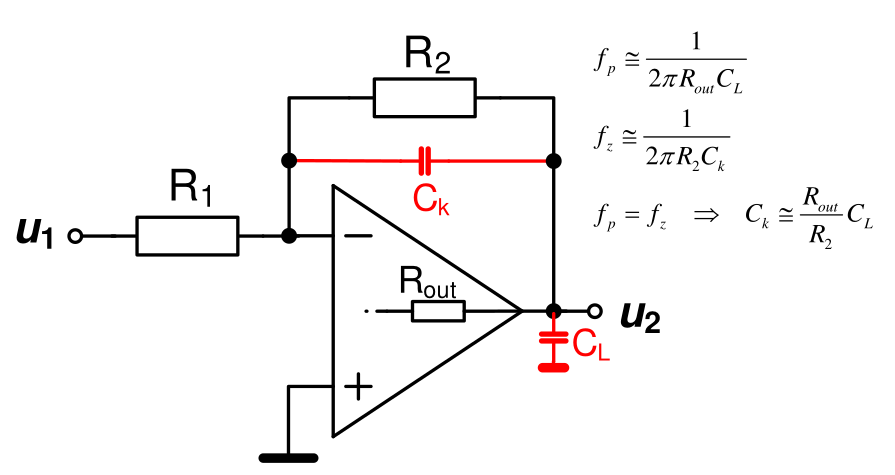
\includegraphics[width=0.5\linewidth]{Obrazky/AE2/3otazka/korekcnaKapacitaVZV}
	\caption{Korekčná kapacita v spätnej väzbe.}
	\label{fig:korekcnakapacitavzv}
\end{figure}
\section{Obmedzenie rýchlosti prebehu $\rightarrow$ Slew Rate}
Rýchlosť prebehu definuje najrýchlejšie zmeny ktoré je zariadenie schopné spracovať s ohľadom na zmenu vstupného signálu. Jej konečná rýchlosť súvisí s nelineárnym skreslením $\rightarrow$ dôvodom existencie skreslenia a aj konečnej rýchlosti prebehu je obmedzenie výstupného prúdu diferenčného stupňa zosilňovača, resp. iných častí obvodu.
\begin{figure}[H]
	\centering
	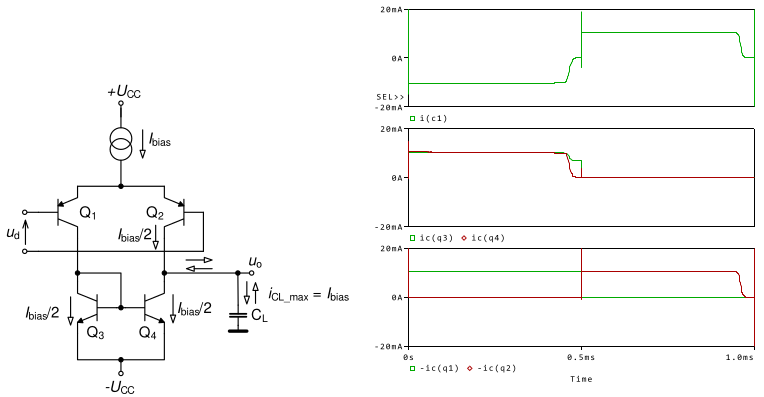
\includegraphics[width=0.55\linewidth]{Obrazky/AE2/3otazka/SRzrkadlo}
	\caption{Diferenčný stupeň so zrkadlom a kapacitnou záťažou.}
	\label{fig:srzrkadlo}
\end{figure}
\begin{description}
	\item[Extrém A] Prebudený vstup uzavrie T1 $\rightarrow$ prúdové zrkadlo nepracuje $\rightarrow$ celý $I_{bias}$ tečie cez T2 a nabíja kapacitu $C_L$
	\item[Extrém B] Opačne prebudený vstup uzavrie T2 $\rightarrow$ $I_{bias}$ tečie cez T1, to otvára prúdové zrkadlo, ktoré vybíja kapacitu $C_L$
\end{description}
\begin{itemize}
	\item Rýchlosť prebehu je obmedzená javmi pri nabíjaní kapacít spôsobenými obmedzením náboja na kapacite. Maximálny nárast náboja je obmedzený.
	\item SR je obmedzené najväčšou možnou zmenou napätia na $C$ za čas, spôsobené maximálnym prúdom ktorý $C$ nabíja
	\item DEF: SR je maximálna zmena výstupného napätia za čas.
	\item \begin{equation}
		SR \approx \frac{\Delta U_0}{\Delta t} = \frac{I_{bias}}{C_L}
	\end{equation}
	\item Ovplyvňujú ho aj kapacity v záťaži obvodu.
	\item SR je definované uzlom ktorý má najmenší pomer $\frac{I_{bias}}{C_L}$.
	\item Skreslenie SR sa zamedzí ak: \begin{equation}
		f_{max} = \frac{SR}{2\pi U_{out}}
	\end{equation}
	\item Skreslenie sa prejavuje tak, že pri harmonickom vstupnom signále sa na výstup dostavuje trojuholník $\rightarrow$ toto je extrémny prípad.
	\item Voči SR sa nedá bojovať zápornou spätnou väzbou $\rightarrow$ nakoľko tá by len vrátila skreslený signál na vstup.
\end{itemize}
\section{Šumy v OZ}
\begin{itemize}
	\item Šum ako taký má náhodný charakter a je definovaný gaussovským rozložením pravdepodobnosti.
	\item Je definovaný v čase aj v šírke pásma
	\item \textbf{Trochu symboliky:}
	
	\begin{description}
		\item[$u_N(t)$] - hodnota k $1\text{ Hz}$ (efektívna hodnota šumu = smerodajná odchýlka), v podstate efektívna hodnota šumu v pásme $1\text{ Hz}$.
		\item[$U_N(t)$] - hodnota ku konkrétnej šírke pásma.
		\item[$u_{\text{noise}}(t)$] – okamžité napätie šumu.
		\item[$u_N^2(t)$] - "stredný" šumový výkon (na odpore $1\ \Omega$).
	\end{description}
\end{itemize}
\begin{figure}[H]
	\centering
	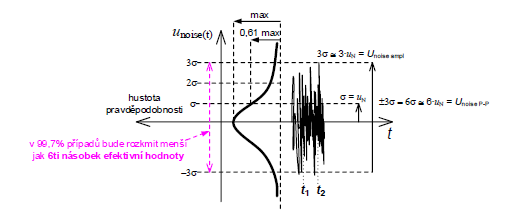
\includegraphics[width=0.7\linewidth]{Obrazky/AE2/3otazka/sumVOZ}
	\caption{Náhodný charakter šumu, výstrelový a biely, jeho statický popis}
	\label{fig:sumvoz}
\end{figure}
Stredná hodnota šumu:
% Stredná kvadratická hodnota šumu
$$u_N^2 = \overline{u_N^2} = \frac{1}{t_2 - t_1} \int_{t_1}^{t_2} u_{\text{noise}}^2(t) \, \text{d}t$$

% Efektívna hodnota šumu
Efektívna hodnota šumu:
$$u_N = \sqrt{\frac{1}{t_2 - t_1} \int_{t_1}^{t_2} u_{\text{noise}}^2(t) \, \text{d}t}$$

% Šumová výkonová a prúdová hustota
Výkonové hodnoty šumu:
$$u_N^2 = \frac{U_N^2}{B} \left[ \frac{\text{V}^2}{\text{Hz}} \right] ; \quad i_N^2 = \frac{I_N^2}{B} \left[ \frac{\text{A}^2}{\text{Hz}} \right]$$

% Spektrálna hustota šumového napätia
Spektrálna hustota šumu:
$$u_N = \frac{U_N}{\sqrt{B}} \left[ \frac{\text{V}}{\sqrt{\text{Hz}}} \right]$$

\begin{figure}[H]
	\centering
	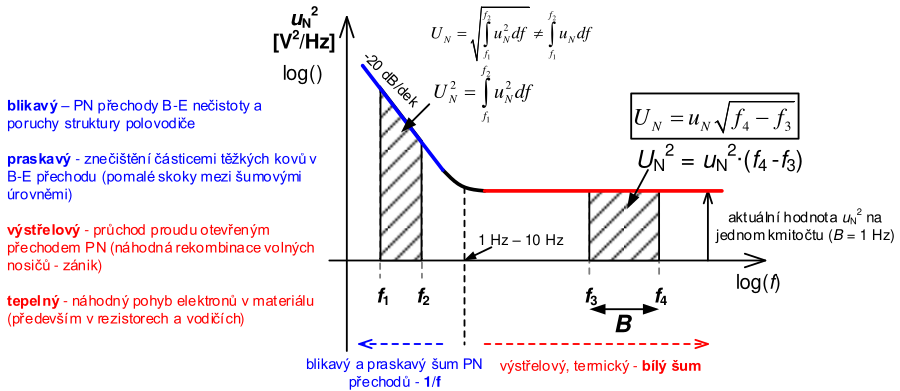
\includegraphics[width=0.7\linewidth]{Obrazky/AE2/3otazka/vykonovaSpektralnaHustotaZdrojeSumu}
	\caption{Výkonová spektrálna hustota a zdroje šumov v obvode.}
	\label{fig:vykonovaspektralnahustotazdrojesumu}
\end{figure}

Šumové pásmo sa rozdeľuje na oblasť pomalých dejov $\frac{1}{f}$, a oblasť bieleho $\rightarrow$ výstrelového šumu.
Výkon šumu závisí na šírke pásma, pričom celková šírka pásma nie je rovná šírke pásma pre pokles o \qty{-3}{\dB}, ale počíta sa z rovností plôch pod ideálnou obdĺžnikovou frekvenčnou charakteristikou:
\begin{equation}
	B_N = \frac{1}{\left|K_{max}\right|} \int_{0}^{\infty} \left|K(f)\right| \,df
\end{equation}
Zdroje šumu sa dajú zrátať dokopy len prostredníctvom výkonu $\rightarrow$ nakoľko majú náhodný charakter, nie sú korelované, nemajú orientáciu.
\begin{figure}[H]
	\centering
	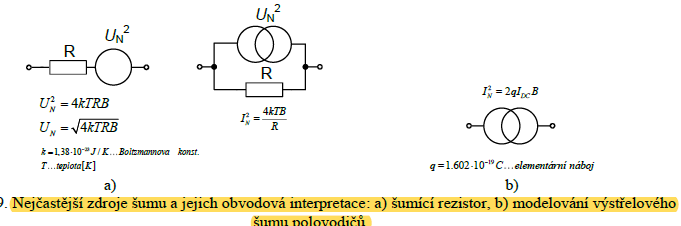
\includegraphics[width=0.7\linewidth]{Obrazky/AE2/3otazka/zdrojeSumuVobvode}
	\caption{Zdroje šumu v obvodoch pre modelovanie}
	\label{fig:zdrojesumuvobvode}
\end{figure}
Šumy v rámci OZ:
\begin{itemize}
	\item V rámci OZ existuje mnoho zdrojov šumu $\rightarrow$ všetky sa uvažujú naraz na výstupe.
	\item Pre zníženie šumu je výhodné používať nízkoimpedančné zdroje signálu $\rightarrow$ veľký odpor má veľký tepelný šum, pričom prevádza prúdové šumy zo vstupu OZ na napätie.
	\item OZ s unipolárnym vstupným párom má nižšie úrovne šumu
	\item Pre nižší šum je vhodné používať čo najmenej rezistorov.
	\item Šumové vlastnosti dvojbranu sú definované šumovým číslom $NF$ (noise figure) v [dB].
	\subitem Toto číslo definuje koľkokrát sa zmenší SNR na vstupe OZ oproti SNR na výstupe OZ.
	\item \begin{equation}
		NF = 20 \log \left[\frac{\frac{U_{sig}}{U_{noise}}\text{in}}{\frac{U_{sig}}{U_{noise}}\text{out}}\right]
	\end{equation}
	\item V kaskádneho radenia existuje Freesov vzťah:
	\item \begin{equation}
		F = F_1 + \frac{F_2 -  1}{A_1} + \frac{F_3 - 1}{A_1 A_2} + \dots + \frac{F_n - 1}{\prod_{i=1}^{n-1} A_{i}}
	\end{equation}
	\item Kedy najväčšie zosilnenie a najväčšie šumové číslo sa umiestňuje do prvého miesta v kaskáde $\rightarrow$ zvyšok má menší vplyv.
\end{itemize}
Ďalšie zdroje šumu:
\begin{itemize}
	\item Parazitné kapacity $\rightarrow$ dá sa potlačiť tienením a usporiadaním
	\item Parazitné induktívne väzby $\rightarrow$ dá sa potlačiť zmenšením rozmerov, skrátením prívodov, zväčšením zemnej plochy
	\item Iskrenie relé a kontaktov v ňom 
	\item Termoeletrické napätia a impulzné špičky $\rightarrow$ dá sa potlačiť teplotnou stabilitou
\end{itemize}
\begin{figure}[H]
	\centering
	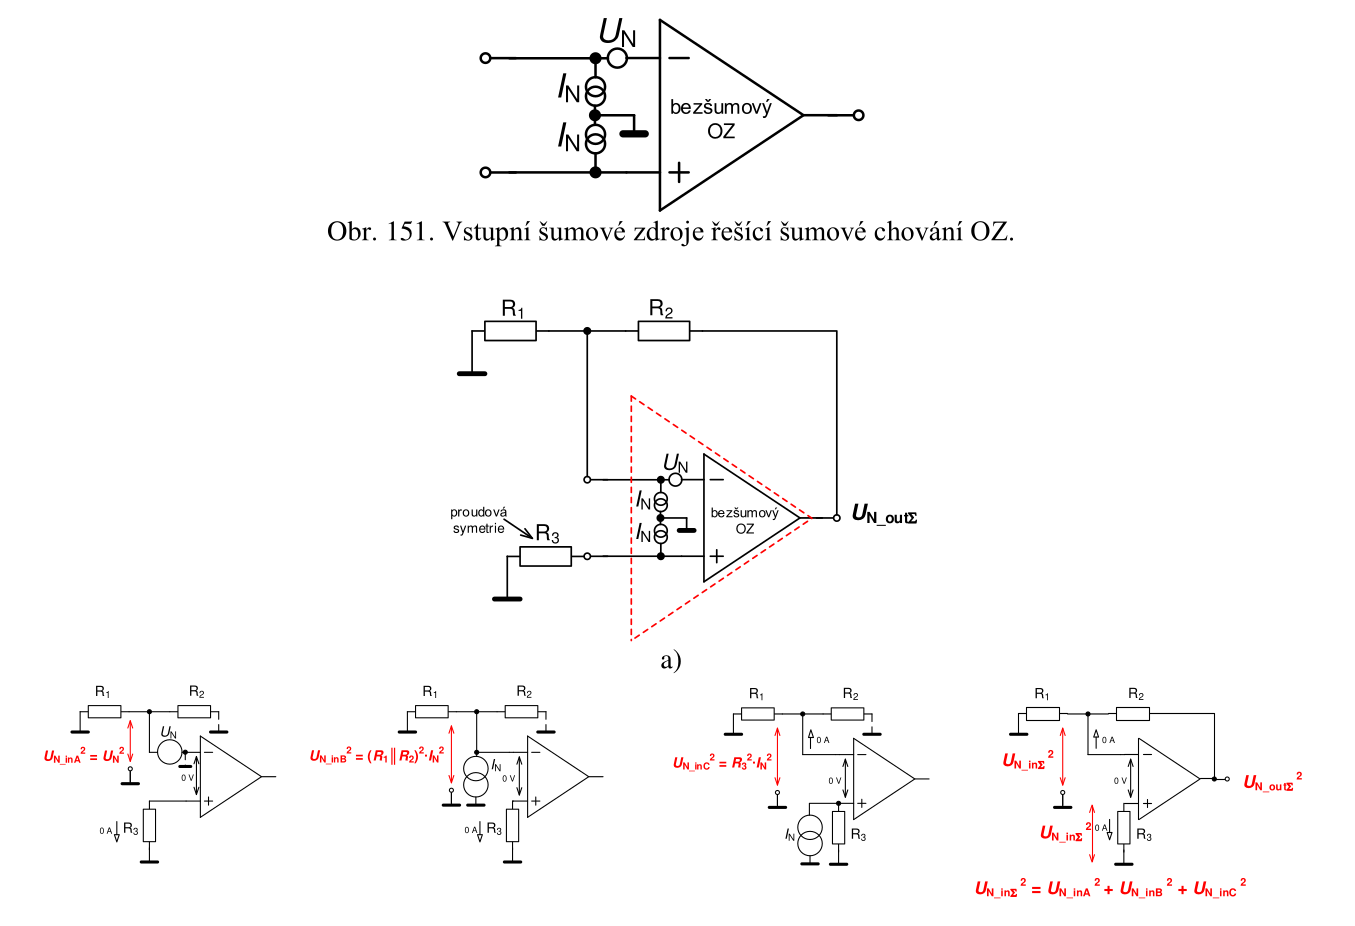
\includegraphics[width=0.9\linewidth]{Obrazky/AE2/3otazka/sumyVoz}
	\caption{Šumová analýza OZ}
	\label{fig:sumyvoz}
\end{figure}
\section{Statická elektrika $\rightarrow$ ochrana proti ESD}
\begin{itemize}
	\item Problémy s ESD vznikajú pri trení povrchov predmetov a plôch.
	\item Pri výboji ESD dochádza k extrémne krátkemu výboju o prúde niekoľko ampér, nanosekundy, s napätiami až niekoľko kV $\rightarrow$ toto nám zabije operák
	\item OZ a integrované obvody obsahujú integrovanú ochranu voči ESD priamo od výrobcov.
	\begin{itemize}
		\item Primárna ochrana
		\subitem Clampy so sériovými rezistormi $\rightarrow$ obmedzenie výbojových prúdov
		\item Sekundárna ochrana
		\subitem Rezistory a clampy chrániace pred vlastnou funkčnou tranzistorovou štruktúrou
		\subitem V prípade, že ochrany nie sú dostatočne rýchle môže sa použiť iný ochranný prvok v rámci silikónu $\rightarrow$ \emph{ESDCGNMOS}.
		\subitem Vysoké hodnoty ochranných rezistorov spôsobujú šum, preto sa rozdeľujú veľké hodnoty do niekoľkých menších hodnôt.
		\subitem Pri rýchlych RF obvodoch sa však požiadavky na ESD zrážajú s požiadavkami na rýchlosť a šírku pásma $\rightarrow$ je nutný kompromis.
	\end{itemize}
	\item Odolnosť MOSFET súčiastok je voči ESD menšia ako JFET a BJT
\end{itemize}
Zásady pri práci s ESD citlivými súčiastkami:
\begin{itemize}
	\item Prepravovať vo fixnom nevodivom prostredí, ideálne so skratovanými vývodmi.
	\item Nechytať sa vývovod.
	\item Pracovný odev bez syntetických vlákien.
	\item Uzemniť sa.
\end{itemize}
\begin{figure}[H]
	\centering
	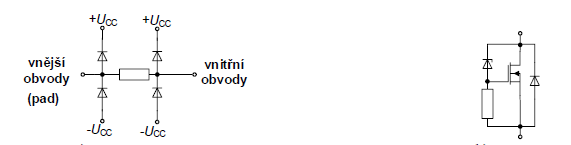
\includegraphics[width=0.7\linewidth]{Obrazky/AE2/3otazka/ochranaESD}
	\caption{Primárna Clamp ochrana a rýchly ESDCGNMOS.}
	\label{fig:ochranaesd}
\end{figure}
\section{Ochrana vstupov, výstupov a napájania OZ voči prepólovaniu, a skratom}
\begin{itemize}
	\item Jedná sa o ochranu pred nedovolenou napäťovou úrovňou, obmedzenie výstupného prúdu
	\item Ochrana voči prepólovaniu: Zapojenie ochranných diód do série s napájaním.
	\item Ochrana vstupov so štandardnou spätnou väzbou $\rightarrow$ antiparalelné zapojenie diód $\rightarrow$ diferenčné napätie.
	\item Používajú sa rýchle spínacie diódy $\rightarrow$ diódy delinearizujú vstupný odpor a nesmú reagovať až príliš
	\item V prípade, že zosilňovač pláva $\rightarrow$ je nutné zaistiť ochranu voči common-mode napätí.
	\subitem Zhoršenie vstupného odporu a common mode rejection ratio.
	\subitem Zhoršenie je dané kvalitou diód.
\end{itemize}
\begin{figure}[H]
	\centering
	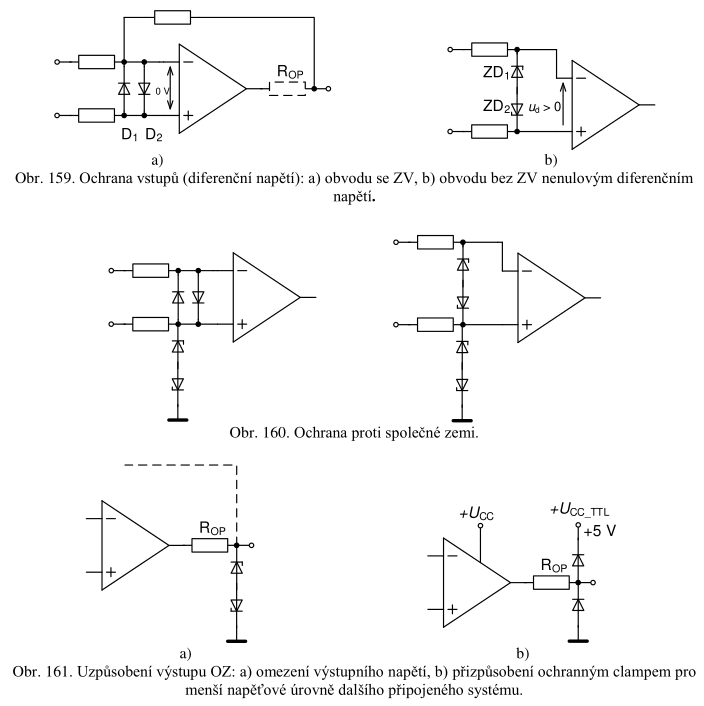
\includegraphics[width=0.7\linewidth]{Obrazky/AE2/3otazka/ochranaVstupov}
	\caption{}
	\label{fig:ochranavstupov}
\end{figure}
\section{Napájanie OZ}
\begin{itemize}
	\item Väčšina OZ vyžaduje a aj má symetrické napájanie
	\subitem V prípade, že nie je dostupné symetrické napájanie $\rightarrow$ vytvorí sa umelá zem v polovičke napájacej hladiny $\rightarrow$ toto môže znamenať problém, nakoľko zem môže plávať s teplotou ak je vytvorená deličom a pod.
	\subitem Vytvára sa z deliča alebo z presných referenčných zdrojov $\rightarrow$ zennerových diód.
	\begin{figure}[H]
		\centering
		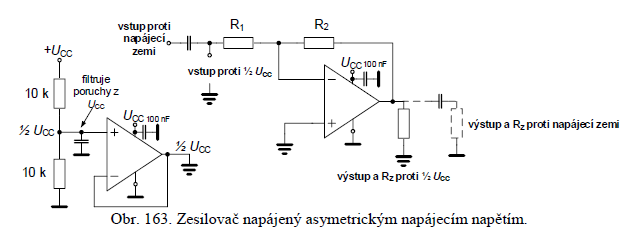
\includegraphics[width=0.7\linewidth]{Obrazky/AE2/3otazka/umelaZem}
		\caption{Umelá zem.}
		\label{fig:umelazem}
	\end{figure}
	\subitem Je potrebné použiť napäťový sledovač $\rightarrow$ pri použití čisto analógovej zeme je obvod po istú dobu po zapnutí nefunkčný, treba OZ.
	\item Dôležitým je správne usporiadanie napájania a zemí $\rightarrow$ najväčší konštrukčný problém.
	\item Napájacia vetva musí mať ideálne nulovú impedanciu $\rightarrow$
	\subitem Inak sa objavujú vplyvy šumu, kmitanie, citlivosť na zmeny v napájacom napätí
	\item Citlivosť na zmeny v napájacom napätí $\rightarrow$ PSRR $\rightarrow$ Power Supply Rejection Ratio
	\subitem Klesá so zvyšujúcou sa frekvenciou
	\subitem Vďaka tomu sa z napájania môže dostať do obvodu VF rušenie pochádzajúce zo zdroja
	\item Obrana voči šumu z napájania $\rightarrow$ blokovací kondenzátor.
	\subitem Pri krátkodobých nárastoch odberu prúdu poskytuje potrebnú energiu.
	\subitem Pracuje aj ako filtre pre VF zložky, ktoré skratuje na zem.
	\subitem Ideálne keramický kondík $\rightarrow$ má nižšie indukčnosti.
	\item Pri použití blokovacích kondenzátorov sa vytvára induktívna slučka vďaka prúdu ktorý tečie z kondíka do obvodu.
	\subitem Pre zamedzenie induktívnych slučiek je potrebné skrátiť vzdialenosti medzi kondíkom, napájaním, zemou a zariadením.
	\begin{figure}[H]
		\centering
		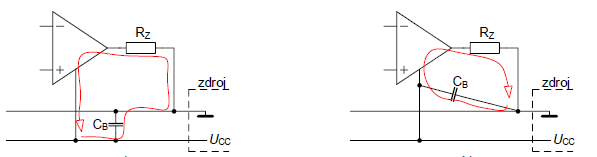
\includegraphics[width=0.7\linewidth]{Obrazky/AE2/3otazka/kondikKratka}
		\caption{Skrátenie induktívnej slučky.}
		\label{fig:kondikkratka}
	\end{figure}
	\item Zemnenie je ďalší problém
	\subitem Zem musí mať zanedbateľnú indukčnosť a čo najmenší odpor
	\subitem Realizuje sa zemniaca plocha pre všeobecnú zem
	\subitem V prípade, že sa uzatvárajú veľké prúdy zemou $\rightarrow$ je potrebné viesť cesty zvlášť $\rightarrow$ rušenie.
	\subitem Ideálna zem neexistuje $\rightarrow$ záleží na veľkosti prúdov
	\subitem Môže dochádzať aj k vytvoreniu kladnej ZV $\rightarrow$ oddelenie zemí a spojenie v inom mieste $\rightarrow$ iná cesta pre signál a pre prúdy.
	\begin{figure}[H]
		\centering
		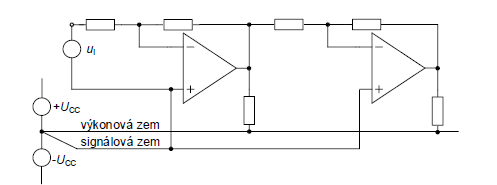
\includegraphics[width=0.7\linewidth]{Obrazky/AE2/3otazka/umelaZem1}
		\caption{Rozdelenie zemí}
		\label{fig:umelazem1}
	\end{figure}
	\item Skurvená parazitná kapacita vstupu voči zemi:
	\subitem Môže spôsobiť nárast zosilnenia na vysokých frekvenciách $\rightarrow$ vytvára parazitný pól
	\subitem Vysoké prevýšenie zisku $\rightarrow$ tvorí oscilácie $\rightarrow$ kompenzačná kapacita a tlmenie činiteľa akosti pomocou odporu
	\begin{figure}[H]
		\centering
		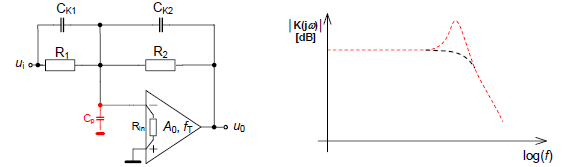
\includegraphics[width=0.7\linewidth]{Obrazky/AE2/3otazka/umelaZem2}
		\caption{Parazitná kapacita na vstupe}
		\label{fig:umelazem2}
	\end{figure}
	
\end{itemize}\section{Diferenčný pár}
\section{Millerov OZ}

\section{Kompenzácia napäťovej a prúdovej nesymetrie OZ}
\begin{itemize}
	\item Reálne OZ sú do istej miery nesymetrické
	\item Majú z výroby prirodzený offset $\rightarrow$ dá sa zistiť pri skratovaní výstupov a meraní napätia na výstupe
	\item Kompenzuje sa privedením opačného napätia na vstup $\rightarrow$ vytvorí sa umelý offset, ktorý kompenzuje ten prirodzený.
	\item Offset je v mV až uV.
	\item Pokiaľ má OZ veľké zosilnenie tak už malý vstupný offset môže saturovať výstup $\rightarrow$ spôsobiť veľkú DC zložku na výstupe
	\item offsetové napätie záleží na teplote $\rightarrow$ teplotný drift súčiastok / offsetu
	\subitem vstupný offset je možné trimmovať laserom pri výrobe
	\begin{figure}[H]
		\centering
		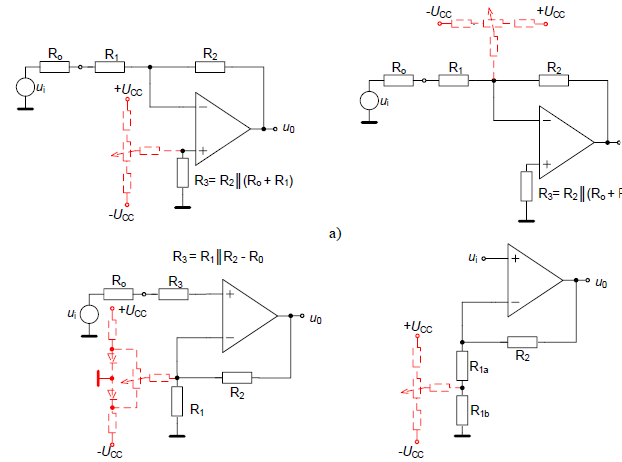
\includegraphics[width=0.5\linewidth]{Obrazky/AE2/3otazka/offsetNapatieKompenzacia}
		\caption{Kompenzácia vstupnej napäťovej nesymetrie.}
		\label{fig:offsetnapatiekompenzacia}
	\end{figure}
	\item Prúdová nesymetria vzniká tým, že OZ má malý vstupný prúd, ktorý je každý iný.
	\item Ich nerovnosti môžu vyvolať rozdiel vstupných napätí
	\item Rieši sa pripojením rezistorov na vstup
	\item Odporové deliče regulujú vstupný prúd inverujúcou a neinvertujúcou vetvou $\rightarrow$ vyrovnávanie prúdov.
\end{itemize}

\section{Diferenčný pár}

\begin{itemize}
	\item Základný stavebný blok OZ.
	\item Prevodník z diferenciálneho vstupného napätia výstupný rozdielový prúd
	\item Je vysoko nelineárny
	\item Existuje bipolárny a unipolárny diferenčný pár.
	\item Tvorí základ pre diferenciálny napäťový zosilňovač
\end{itemize}
\begin{figure}[H]
	\centering
	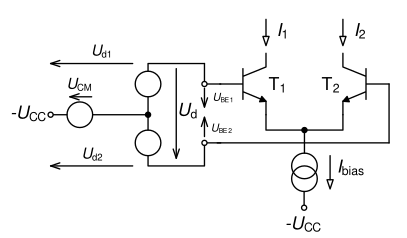
\includegraphics[width=0.5\linewidth]{Obrazky/AE2/3otazka/differ}
	\caption{Bipolárny diferenciálny stupeň pre nelineárnu (veľko signálovú) analýzu.}
	\label{fig:differ}
\end{figure}
Výsledný rozdielový prúd sa dá stanoviť ako:
\begin{equation}
	\Delta I_{out} = I_1 - I_2 = I_{bias}\tanh \left(\frac{U_d}{2U_{TE}}\right)
\end{equation}
Závislosť je jasne nelineárna, v prípade, že $U_d$ je v rozmedzí $\pm 50 \text{ mV}$ môžeme tú závislosť za lineárnu považovať.
\begin{figure}[H]
	\centering
	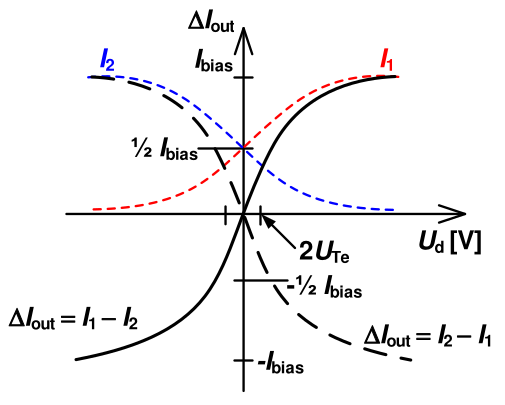
\includegraphics[width=0.3\linewidth]{Obrazky/AE2/3otazka/differZavislost}
	\caption{Prevodová charakterisitka diferenciálneho stupňa.}
	\label{fig:differzavislost}
\end{figure}
\begin{figure}[H]
	\centering
	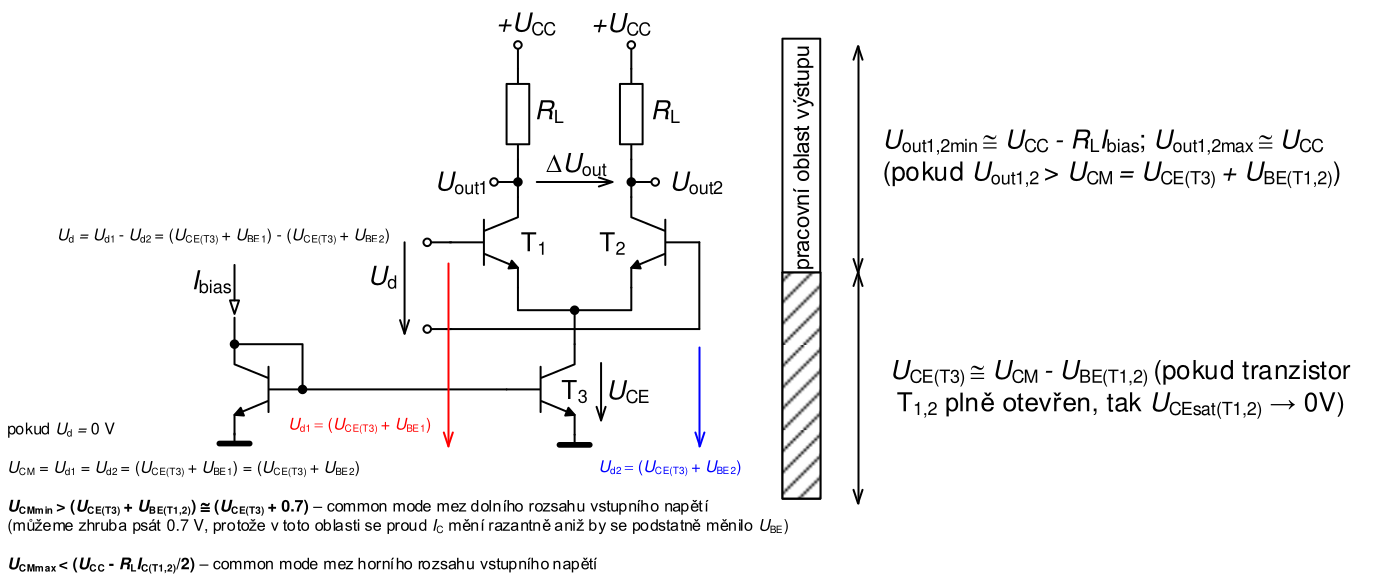
\includegraphics[width=0.75\linewidth]{Obrazky/AE2/3otazka/differZosilnovacSRezZatazou}
	\caption{Diferenčný zosilňovač s rezistívnou záťažou.}
	\label{fig:differzosilnovacsrezzatazou}
\end{figure}
\begin{figure}[H]
	\centering
	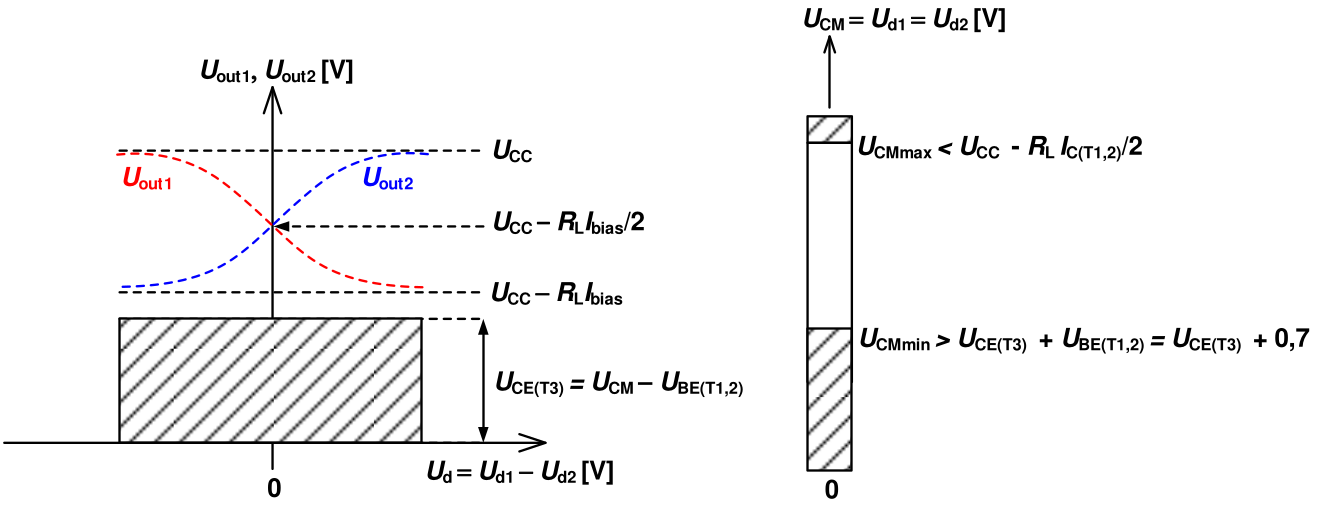
\includegraphics[width=0.7\linewidth]{Obrazky/AE2/3otazka/medzeVstupnychNapatiDiffer}
	\caption{Medze vstupných napätí zosilňovača pre súhlasné napätie vstupov. Statická prevodná charakteristika, medze súhlasného vstupného napätia.}
	\label{fig:medzevstupnychnapatidiffer}
\end{figure}
\begin{figure}[H]
	\centering
	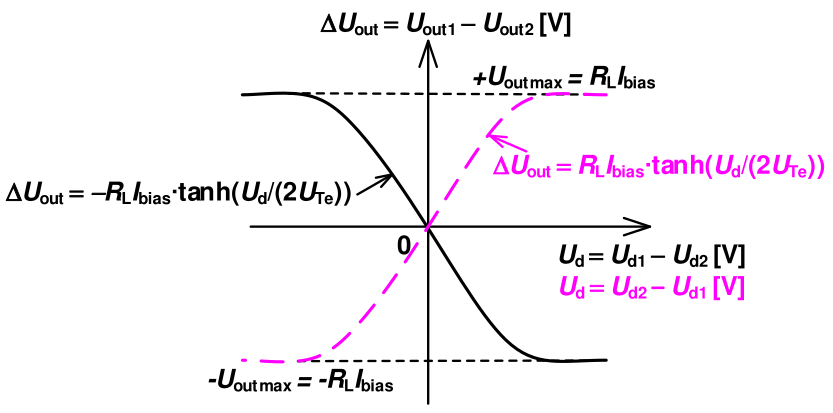
\includegraphics[width=0.4\linewidth]{Obrazky/AE2/3otazka/prevodnaCharakteristikaDiffer}
	\caption{Napäťová prevodná charakteristika.}
	\label{fig:prevodnacharakteristikadiffer}
\end{figure}
\textbf{Diferenciálny zosilňovač je možné linearizovať využitím emitorových degradačných rezistorov.}
\begin{figure}[H]
	\centering
	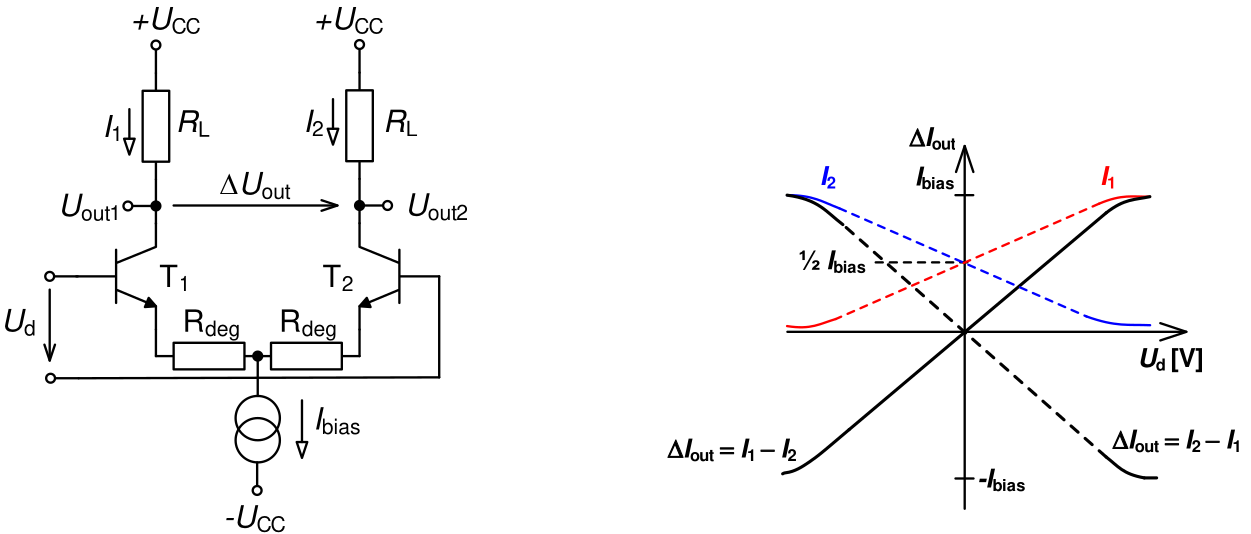
\includegraphics[width=0.7\linewidth]{Obrazky/AE2/3otazka/linearizaciaDiffZosikaVar1}
	\caption{Emitorová degradácia diferenčného zosilňovača.}
	\label{fig:linearizaciadiffzosikavar1}
\end{figure}
\begin{figure}[H]
	\centering
	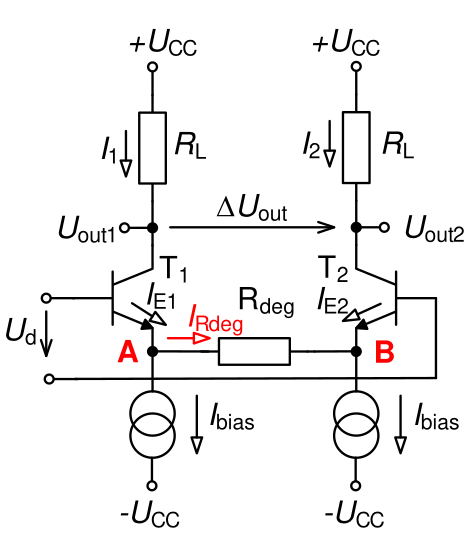
\includegraphics[width=0.3\linewidth]{Obrazky/AE2/3otazka/linearizaciaDiffZosikaVar2}
	\caption{Druhá možnosť emitorovej degradácie diferenčného zosilňovača.}
	\label{fig:linearizaciadiffzosikavar2}
\end{figure}
Ďalej je možná linearizácia pomocou inverznej prevodnej charakteristiky.
\begin{figure}[H]
	\centering
	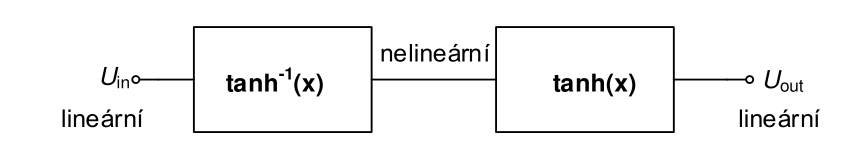
\includegraphics[width=0.35\linewidth]{Obrazky/AE2/3otazka/principLinearizacieInverznouCharakteritikou}
	\caption{Princíp linearizácie pomocou inverznej prevodovej charakteristiky.}
	\label{fig:principlinearizacieinverznoucharakteritikou}
\end{figure}
\begin{figure}[H]
	\centering
	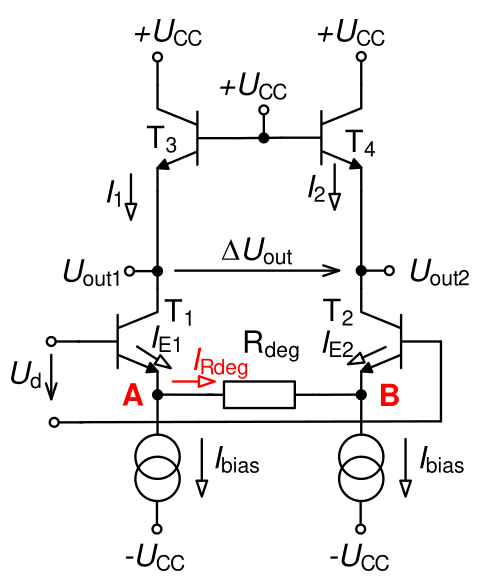
\includegraphics[width=0.3\linewidth]{Obrazky/AE2/3otazka/linearizaciaDiffZosikaVar3}
	\caption{Linearizácia diferenčného zosilňovača s členom funkcie $\tanh^{-1}$}
	\label{fig:linearizaciadiffzosikavar3}
\end{figure}
V praxi sa asi využíva viacero linearizačných techník pre vstup a výstup:
\begin{figure}[H]
	\centering
	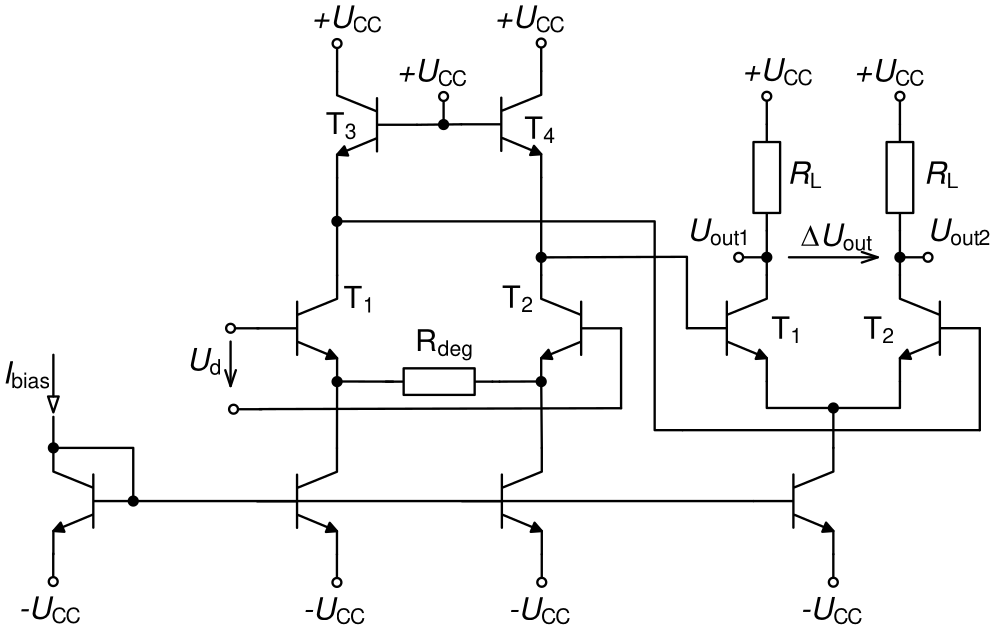
\includegraphics[width=0.7\linewidth]{Obrazky/AE2/3otazka/kompletnaLinearizaciaZosika}
	\caption{Linearizácia diferenčného zosilňovača.}
	\label{fig:kompletnalinearizaciazosika}
\end{figure}
\subsection{Unipolárny diferenciálny pár}
Rovnako ako pre bipolár, je možné skonštruovať aj unipolárnu variantu, závislosť výstupného prúdu je však kvadratická vďaka použitej technológií.
\begin{figure}[H]
	\centering
	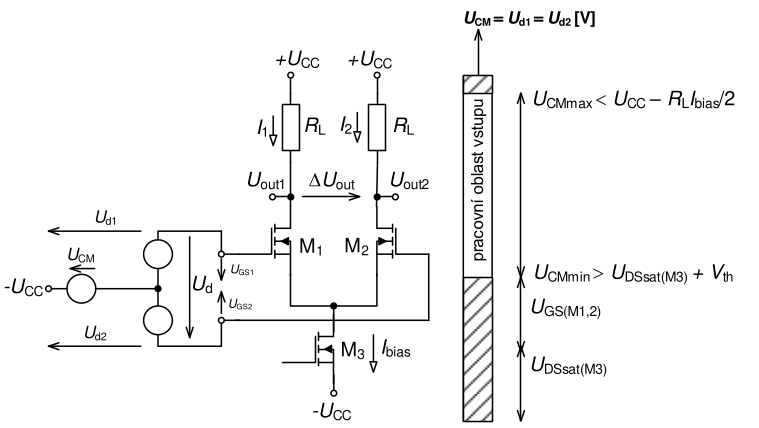
\includegraphics[width=0.7\linewidth]{Obrazky/AE2/3otazka/unipolarLin}
	\caption{Diferenčný zosilňovač s unipolárnym diferenčným párom.}
	\label{fig:unipolarlin}
\end{figure}
Platí, že \begin{equation}
	\Delta i_{out} = \Delta u_d \sqrt{\mu_0 C_{OX} \frac{W}{L} I_{bias}} = \Delta u_d g_m
\end{equation}
\newpage
\section{Millerov OZ}
\begin{itemize}
	\item Má koncový stupeň v triede A
	\item Má niekoľko pólov frekvenčnej charakteristiky $\rightarrow$ sú definované kapacitami vysokoimpedančných uzlov
	\item Bez zásahu nie je žiaden z týchto pólov dominantný na nízkych frekvenciách $\rightarrow$ teda je nestabilný
	\item Stabilita je daná Millerovou kompenzačnou kapacitou v spätnej väzbe $C_M$
	\item Využíva millerovho javu $\rightarrow$ pokiaľ je zapojená v spätnej väzbe tak je transformovaná na ekvivalentnú kapacitu ktorej hodnota už odpovedá kapacite pôvodnej $C_M$ ktorá je zosilnená o stupeň $M_5$
	\item Tranzientná frekvencia je daná zhruba tou kapacitou millerovho javu: \[\text{GBW} = f_{d1} A_U\]
	\item $C_M$ samá o sebe tvorí aj nulu v prenose, tá nám tú stabilitu ešte viac dojebáva, šak prečo nie $\rightarrow$ preto sa vkladá do série odpor $R_M$ s $C_M$ a nula magicky zmizne (boha toto sú kokotiny)
	\item Výstupné napätie na prázdno sa bude nachádzať medzi napájacími limitmi zníženými o saturačné úbytky na výstupných tranzistoroch
\end{itemize}
\begin{figure}[H]
	\centering
	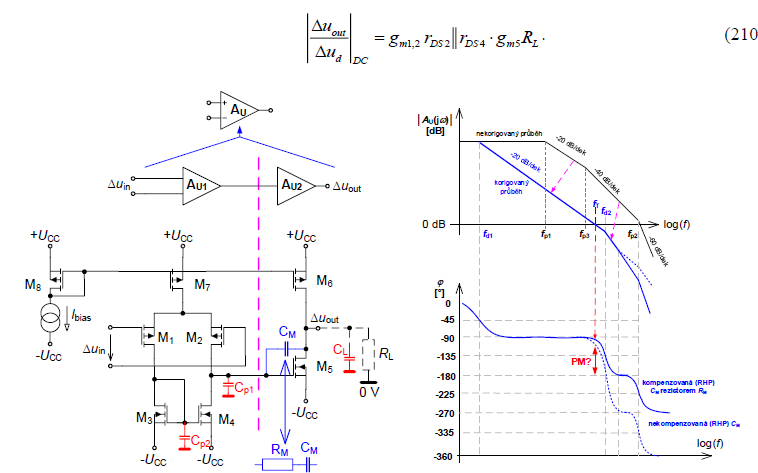
\includegraphics[width=0.7\linewidth]{Obrazky/AE2/3otazka/miller}
	\caption{Millerov dvojstupňový zosilňovač.}
	\label{fig:miller}
\end{figure}
